%\author{\href{https://bit.ly/lorentztransformation}{Google AI studio prompt}\\ \small \emph{Derivado de los Postulados de la Relatividad Especial}}

\documentclass[11pt,a4paper]{article}

% --- PAQUETES ---
\usepackage[margin=1in]{geometry} % Establecer márgenes de página
\usepackage{amsmath}              % Para entornos matemáticos avanzados como aligned, pmatrix, boxed
\usepackage{amssymb}              % Para símbolos matemáticos adicionales
\usepackage{graphicx}             % Para incluir gráficos
\usepackage{cancel}    
\usepackage[dvipsnames]{xcolor}
\usepackage{hyperref}             % Para hipervínculos y metadatos del PDF
\hypersetup{
    colorlinks=true,
    linkcolor=blue,
    filecolor=magenta,      
    urlcolor=cyan,
    pdftitle={Derivación de las Transformaciones de Lorentz},
    pdfauthor={Asistente de IA},
    bookmarks=true,
    pdfpagemode=UseOutlines,
}
\usepackage{enumitem}
\usepackage{tikz}
% https://www.texdev.net/2021/06/30/siunitx-v2-to-v3
\usepackage{siunitx}
\renewcommand{\arraystretch}{1.9}
% commment/uncomment to show/hide the solution
%\renewcommand{\phantom}[1]{#1}

% --- INFORMACIÓN DEL TÍTULO ---
\title{Una Derivación Completa de las Transformaciones de Lorentz \\ y su Interpretación Geométrica}
\author{\href{https://bit.ly/lorentztransformation}{Google AI studio prompt}\\ \small \emph{Derivado de los Postulados de la Relatividad Especial}}
\date{\today}

% --- INICIO DEL DOCUMENTO ---
\begin{document}

\maketitle
\tableofcontents


\begin{abstract}
Este documento proporciona una derivación detallada y paso a paso de las transformaciones de Lorentz, fundamentada en los postulados de la Relatividad Especial. Luego, extiende esta derivación para explorar la estructura geométrica más profunda de las transformaciones, introduciendo los conceptos de rapidez y el formalismo matricial. Finalmente, demuestra cómo un impulso de Lorentz (boost) puede ser visto formalmente como una rotación en un espaciotiempo complejo a través de una rotación de Wick.
\end{abstract}

\section{Introducción}

Las transformaciones de Lorentz son la piedra angular de la teoría de la Relatividad Especial de Einstein. Relacionan las coordenadas de espacio y tiempo de un evento según lo medido por dos observadores en diferentes sistemas de referencia inerciales. Reemplazan a las antiguas transformaciones de Galileo, que son inconsistentes con la constancia observada de la velocidad de la luz.

La derivación se basa en dos postulados fundamentales de la Relatividad Especial:
\begin{enumerate}
    \item \textbf{El Principio de Relatividad:} Las leyes de la física son las mismas en todos los sistemas de referencia inerciales.
    \item \textbf{La Constancia de la Velocidad de la Luz:} La velocidad de la luz en el vacío, denotada por $c$, es la misma para todos los observadores inerciales, independientemente del movimiento de la fuente de luz o del observador.
\end{enumerate}

El segundo principio puede ser cambiado simplemente por la suposición de que el espacio y el tiempo deben ser homogéneos e isotrópicos, ver \url{https://arxiv.org/pdf/gr-qc/0107091}

La motivación de la relatividad especial surge de la necesidad de usar el primer postulado para la interacción electromagnética. Aunque dicho postulado es evidente en sistemas mecánicos, no es claro para la interacción electromagnética. De hecho, una partícula cargada en reposo sólo tiene asociado un campo eléctrico, mientras que una partícula moviéndose a velocidad constante relativa al observador en reposo, genera una corriente eléctrica que a su vez induce un campo magnético. Además, el campo eléctrico se deforma (las regiones de campo constante pasan de ser esféricas a elipsoidales). Cómo en última instancia los objetos de medida están hechos de partículas cargadas dentro de los átomos que la componen, es de esperarse

\section{Preliminares}

\subsection{Vectores en Dos Dimensiones}

Un \textbf{vector} es una cantidad que tiene tanto \textbf{magnitud} (tamaño) como \textbf{dirección}. En dos dimensiones, un vector se puede representar como una flecha en un plano.  La longitud de la flecha representa la magnitud, y la orientación de la flecha representa la dirección.  Matemáticamente, podemos expresar un vector en dos dimensiones como un par ordenado de números (componentes), por ejemplo, $(x, y)$, donde:
\begin{itemize}
    \item $x$ es la componente horizontal del vector.
    \item $y$ es la componente vertical del vector.
\end{itemize}

\subsubsection{Cálculo de Magnitud Dirección}

\begin{tikzpicture}[scale=0.9]
    % Ejes
    \draw[->] (-1,0) -- (5,0) node[right] {$x$};
    \draw[->] (0,-1) -- (0,4) node[above] {$y$};

    % Vector v
    \coordinate (O) at (0,0);
    \coordinate (V) at (3,2);
    \coordinate (W) at (0,2);
    \draw[->, thick, blue] (O) -- (V) node[midway, above right] {$\boldsymbol{v} = (x, y)$};

    % Coordenadas y líneas auxiliares
    \coordinate (X) at (3,0);
    \draw[dashed] (V) -- (X);
    \draw[dashed] (V) -- (W);
    \draw (0,0) -- (X);
    \node[below] at (X) {$x$};
    \node[left] at (0,2) {$y$};

    % Ángulo
    \draw[<->] (0.7,0) arc (0:33.69:0.7);
    \node at (1.2,0.4) {$\theta$};

    % Etiquetas
    \node[below left] at (O) {$O$}; % Origen
    %\node[right] at (V) {$V$}; % Extremo del vector

    %Cálculo de ángulo:
    \node[right] at (3.7,1) {$\tan\theta = \dfrac{y}{x}$};
\end{tikzpicture}

La magnitud del vector viene dada por la longitud del vector, que corresponde a la hipotenusa del triángulo rectángulo de lados $x$ y $y$, se denota por $|\boldsymbol{v}|$ o simplemente $v$
\begin{align}
    v = \sqrt{x^2+y^2}\,.
\end{align}



El ángulo $\theta$ que define la dirección del vector está dado por:

$$\theta = \arctan{\left(\frac{y}{x}\right)}$$

\subsubsection{Ejemplos de Vectores en Física}

\subsubsection{Posición}
\begin{itemize}
    \item \textbf{Concepto:} Indica la ubicación de un objeto en un plano.
    \item \textbf{Ejemplo:} Un robot se encuentra en un plano cartesiano. Su posición está descrita por el vector $\textbf{r} = (3, 4)$ metros. Esto significa que el robot está a 3 metros a la derecha del origen y a 4 metros hacia arriba del origen.
    \item \textbf{Magnitud:} La distancia del robot al origen, $|\textbf{r}|=\sqrt{3^2+4^2}= 5$ metros.
    \item \textbf{Dirección:} El ángulo que forma la flecha con el eje horizontal, cuyo cálculo involucraría funciones trigonométricas (arctan(4/3)).
\end{itemize}

\subsubsection{Velocidad}
\begin{itemize}
    \item \textbf{Concepto:} Describe qué tan rápido y en qué dirección se mueve un objeto.
    \item \textbf{Ejemplo:} Un drone vuela a 10 m/s en un ángulo de 30 grados hacia el noreste. La velocidad se representa como $\textbf{v} = (8.66, 5)$ m/s (aproximadamente).
    \item \textbf{Magnitud:} La rapidez del drone es 10 m/s.
    \item \textbf{Dirección:} 30 grados hacia el noreste.
\end{itemize}

\subsubsection{Aceleración}
\begin{itemize}
    \item \textbf{Concepto:} Describe la tasa de cambio de la velocidad.
    \item \textbf{Ejemplo:} Un carro que se mueve hacia el este aumenta su velocidad en la dirección horizontal, por lo que su aceleración es $\textbf{a} = (2, 0)$ m/s$^2$.  Esto indica que su velocidad horizontal aumenta en 2 m/s cada segundo, mientras que su velocidad vertical no cambia.
    \item \textbf{Magnitud:} 2 m/s$^2$
    \item \textbf{Dirección:} Hacia el este.
\end{itemize}

\subsubsection{Fuerza}
\begin{itemize}
    \item \textbf{Concepto:} Una influencia que puede causar que un objeto cambie su movimiento (acelere).
    \item \textbf{Ejemplo:} Una persona empuja una caja en diagonal, aplicando una fuerza de $\textbf{F} = (5, -3)$ N.  Esto significa que la persona está empujando con 5 Newtons hacia la derecha y 3 Newtons hacia abajo.
    \item \textbf{Magnitud:} $|\textbf{F}|=\sqrt{5^2+(-3)^2} = \sqrt{34}$ N
    \item \textbf{Dirección:} Hacia la derecha e inclinado hacia abajo (el ángulo se calcularía con la función arcotangente).
\end{itemize}

\subsubsection{Operaciones con Vectores}

\begin{itemize}
    \item \textbf{Suma de Vectores:} Sumar las componentes correspondientes de cada vector.
    \item \textbf{Multiplicación por un Escalar:} Multiplicar cada componente del vector por el escalar.
    \item \textbf{Magnitud de un Vector:} Usar el teorema de Pitágoras: $|\textbf{v}|=\sqrt{x^2+y^2}$
\end{itemize}


\begin{tikzpicture}[scale=0.8]

    % Ejes
    \draw[->] (0,0) -- (5,0) node[right] {$x$};
    \draw[->] (0,0) -- (0,4) node[above] {$y$};
    \node[below left] at (0,0) {O};

    % Vector v
    \coordinate (V) at (3,1.5);
    \draw[->, thick, blue] (0,0) -- (V) node[midway, above right] {$\boldsymbol{v}$};

    % Vector w
    \coordinate (W) at (2,2.5);
    \draw[->, thick, red] (0,0) -- (W) node[midway, above left] {$\boldsymbol{w}$};

    % Vector Suma (Resultante)
%    \coordinate (Sum) at ($(V)+(W)$); % Calcula la suma
%    \draw[->, ultra thick, green!70!black] (0,0) -- (Sum) %node[midway, above right] {$\boldsymbol{v} + \boldsymbol{w}$};

    % Líneas Guía (Opcional - para ilustrar la regla del paralelogramo)
%    \draw[dashed, gray] (V) -- ($(V)+(W)$);
%    \draw[dashed, gray] (W) -- ($(V)+(W)$);

\end{tikzpicture}

\subsubsection{Importancia}
La representación vectorial nos permite analizar y predecir el movimiento de objetos en el mundo real, donde la dirección es fundamental.  Sin vectores, solo tendríamos magnitudes sin contexto espacial.





\subsection{Simplificacón de unidades}
\begin{table}[h!]
    \centering
    \caption{Cantidades Físicas Fundamentales y sus Unidades SI}
    \begin{tabular}{|l|l|l|}
        \hline
       \textbf{Nombre}           &\textbf{Símbolo}  [Letra] & \textbf{Unidades} (SI) \\ \hline
        Tiempo          & [T]               & segundo (s)   \\ \hline
        Distancia       & [L]               & metro (m)     \\ \hline
        Masa            & [M]               & kilogramo (kg) \\ \hline
        Carga eléctrica & [Q]               & coulomb (C)   \\ \hline
        Temperatura      & [$\Theta$]               & kelvin (K)    \\ \hline
    \end{tabular}
    \label{tab:cantidades_fisicas}
\end{table}

\newpage
Algunas unidades derivadas
\begin{itemize}
\item Magnitud de velocidad y aceleración
\begin{align*}
    [v] =& \left[\dfrac{L}{T}\right]\,, & [a] = \left[\dfrac{L}{T^2}\right]\,
\end{align*}
    \item Magnitud de la fuerza
    \begin{align*}
        F = m a \to [F] =\left[M \dfrac{L}{T^2}\right]
    \end{align*}
    donde $m$ es la masa de una partícula que se mueve con una magnitud de aceleración $a$.
    \item Energía
    A partir de la energía cinética
    \begin{align*}
        E = \frac{1}{2}m v^2 \to [E] = \left[M\frac{L^2}{T^2}\right] \to \text{Joules (J)}
    \end{align*}
    donde $m$ es la masa de la partícula que se mueve con una magnitud de velocidad $v$.
\end{itemize}


En el sistema internacional de unidades tenemos las siguientes cantidades fundamentes

\subsection{Factores de conversión}

\begin{align*}
    1 = \dfrac{\text{cantidad}}{\text{misma cantidad en otras unidades}}
\end{align*}

Ejemplos
\begin{align*}
    1=\dfrac{1\,\text{km}}{1000\,\text{m}} = \dfrac{\text{km}}{1000\,\text{m}} =\dfrac{1000\,\text{m}}{\text{km}}
\end{align*}

Convertir 60 km/h a m/s
\begin{align*}
    60\dfrac{\text{km}}{\text{h}}\cdot 1 =& 60\dfrac{\cancel{\text{km}}}{\text{h}}  \dfrac{1000\,\text{m}}{\cancel{\text{km}}}\\
    =& 60000\dfrac{\text{m}}{\text{h}}\cdot 1\\
    =&60000\dfrac{\text{m}}{\cancel{\text{h}}}
    \dfrac{{\cancel{\text{h}}}}{3600\,\text{s}}\\
    \approx& 16.7 \frac{\text{m}}{\text{s}}
\end{align*}


Ejercicio: Convierta $2\text{m}^2$ a $\text{cm}^2$



\section{Noción de transformaciones}

Un ejemplo de transformación es la de un montaje experimental en la cual se determina el movimiento de un cuerpo con respecto a los ejes $x$, $y$ correspondientes a los lados de la mesa ilustrado en la figura~\ref{fig:tabla} izquierda. Posteriormente se repite la medida con la mesa rotada un ángulo $\theta$ pero manteniendo la posición del montaje experimental sobre la misma, como se ilustra en la figura~\ref{fig:tabla} derecha. Es claro que la trayectoria del movimiento no depende del sistema de referencia.
\begin{figure}
  \centering
  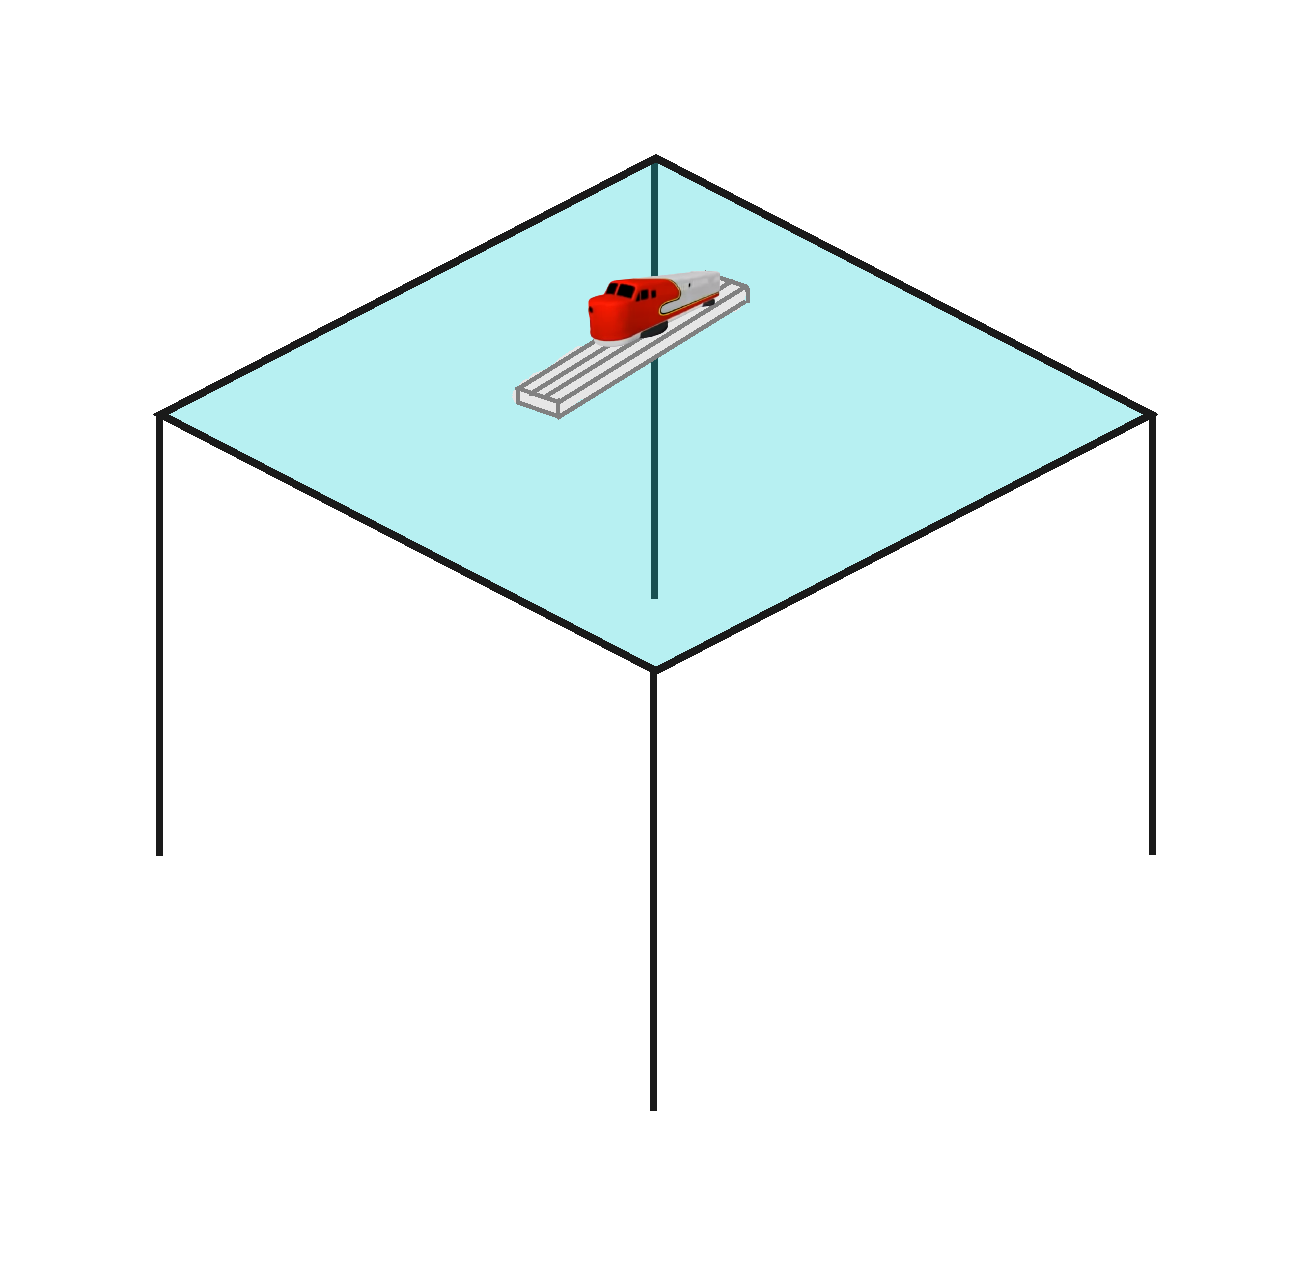
\includegraphics[scale=0.4]{table}
  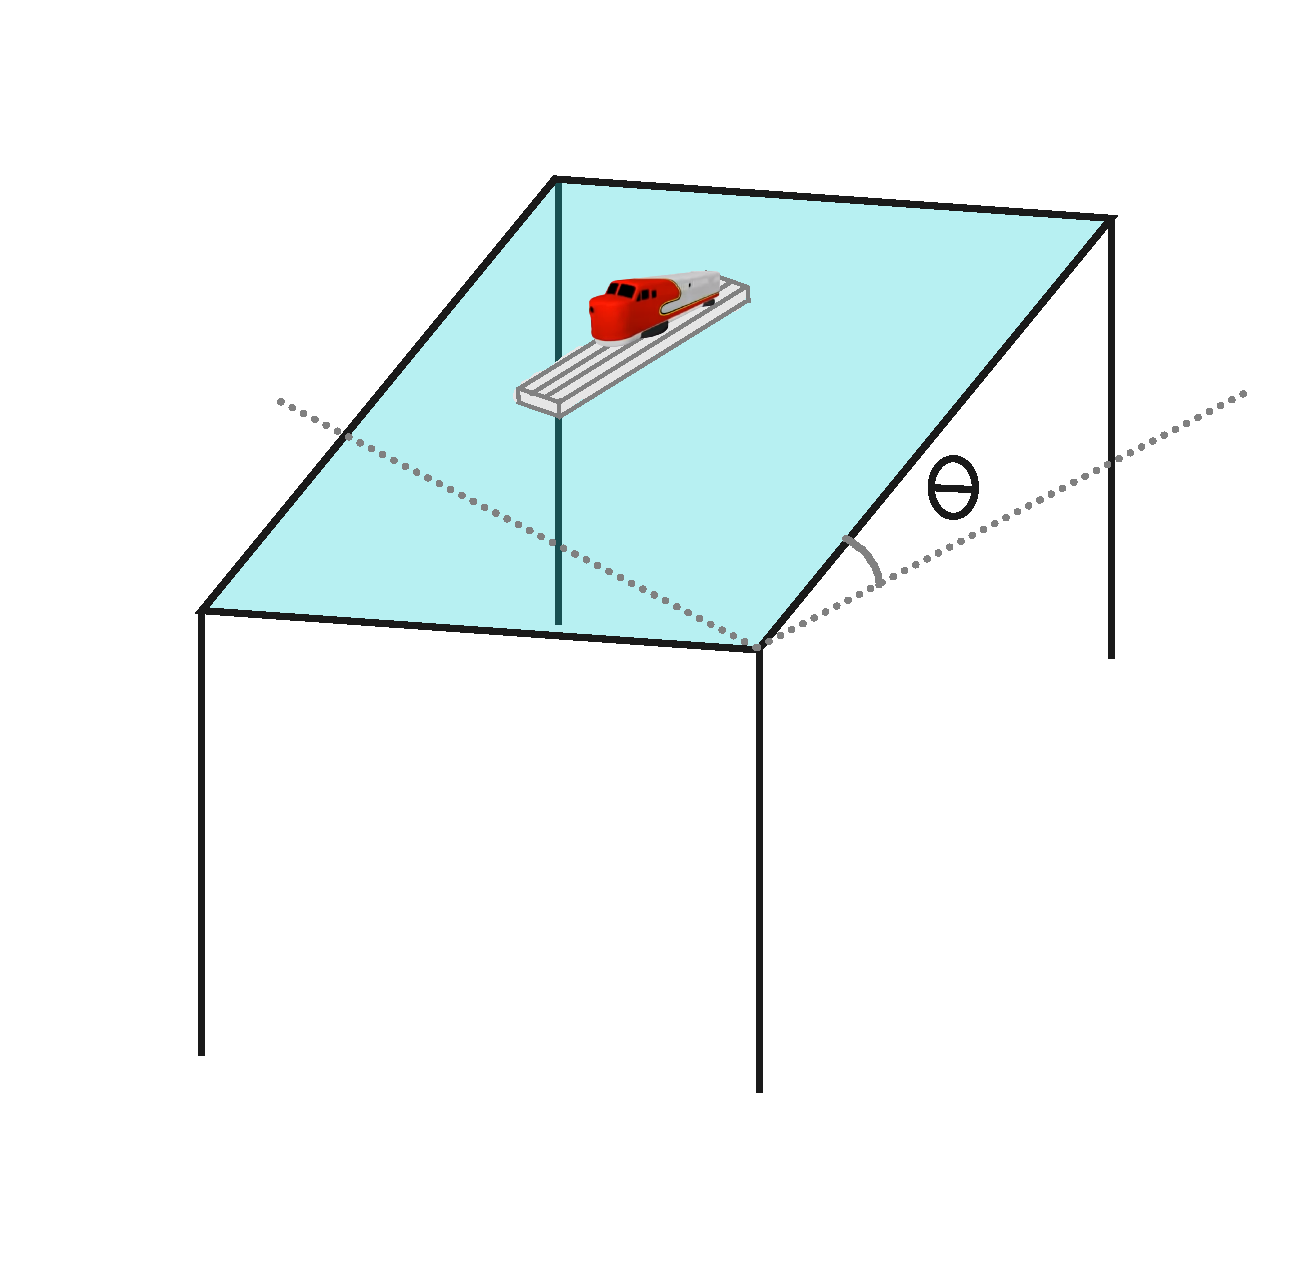
\includegraphics[scale=0.4]{tabletheta}
  \caption{Rotación de sistema de coordenadas}
  \label{fig:tabla}
\end{figure}




\begin{figure}
  \centering
  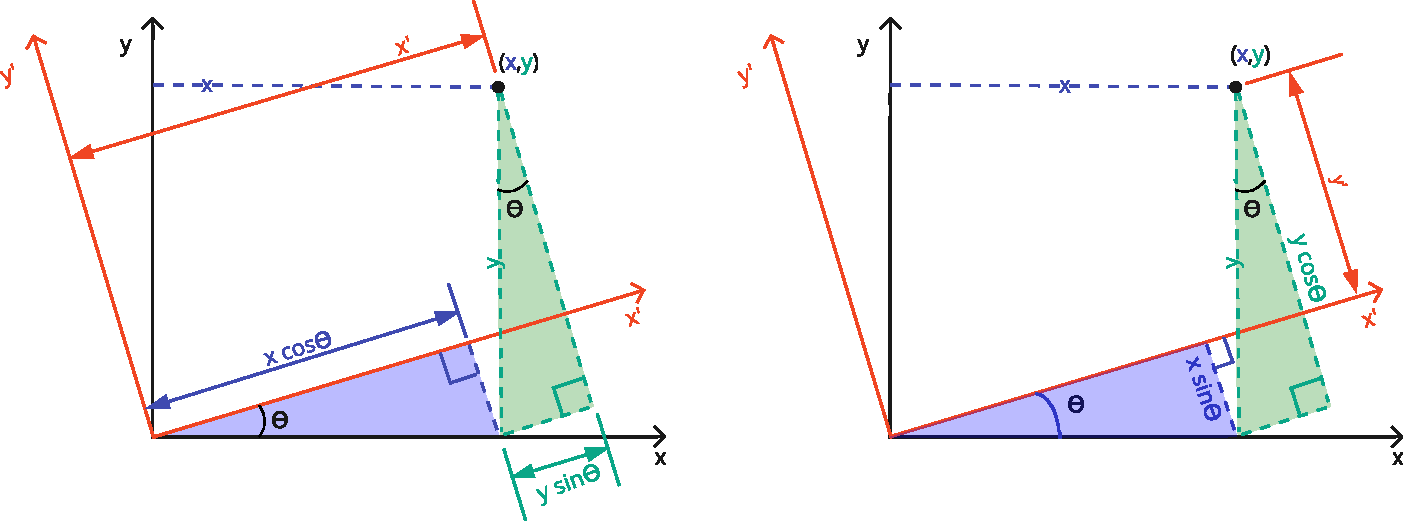
\includegraphics[scale=0.75]{so2}
  \caption{Rotación por ángulo $\theta$}
  \label{fig:so2}
\end{figure}



Considere un punto $(x,y)$ en sistema de referencia de dos dimensiones. Si cambiamos a un sistema de referencia rotado por un ángulo $\theta$, $(x',y')$, como se muestra en la figura~\ref{fig:so2}, podemos definir los dos triángulos rectángulos que se muestran en la figura y a partir de ellos obtener la transformación de los sistemas de referencia debido a la rotación
\begin{align}
  x'=&x\cos\theta+y\sin\theta \nonumber\\
  y'=&y\cos\theta-x\sin\theta\,.
\end{align}

% --- Inicio del código para insertar ---

% Para las ecuaciones matemáticas
\begin{align*}
    \boldsymbol{r} &= (x, y) \\
    \boldsymbol{r}' &= (x', y') \\[1em] % Añade un poco de espacio vertical
    r^2 = \boldsymbol{r} \cdot \boldsymbol{r} &= x^2 + y^2 \\
  {r'}^2 =  \boldsymbol{r}' \cdot \boldsymbol{r}' &= x'^2 + y'^2 = x^2 + y^2 = \boldsymbol{r} \cdot \boldsymbol{r}
\end{align*}

La demostración del último paso se hace a continuación.

% --- Inicio del código para insertar ---

\subsection*{Demostración de la Invariancia del Producto Escalar bajo Rotación}

El objetivo es demostrar que el módulo al cuadrado de un vector es el mismo después de una rotación de coordenadas. Es decir, probaremos que:
\[
\boldsymbol{r}' \cdot \boldsymbol{r}' = \boldsymbol{r} \cdot \boldsymbol{r} \quad \Leftrightarrow \quad x'^2 + y'^2 = x^2 + y^2
\]

\subsubsection*{Paso 1: Ecuaciones de Transformación por Rotación}
Las coordenadas $(x', y')$ en un sistema que ha sido rotado un ángulo $\theta$ en sentido antihorario se relacionan con las coordenadas originales $(x, y)$ mediante:
\begin{align*}
    x' &= x \cos\theta + y \sin\theta \\
    y' &= -x \sin\theta + y \cos\theta
\end{align*}

\subsubsection*{Paso 2: Sustitución y Expansión Algebraica}
Sustituimos estas transformaciones en la expresión para el módulo al cuadrado en el sistema rotado, $\boldsymbol{r}' \cdot \boldsymbol{r}' = x'^2 + y'^2$.

\begin{align*}
    x'^2 + y'^2 &= (x \cos\theta + y \sin\theta)^2 + (-x \sin\theta + y \cos\theta)^2 \\[1em]
    % Expandiendo los binomios al cuadrado
    &= (x^2 \cos^2\theta + 2xy \cos\theta \sin\theta + y^2 \sin^2\theta) \\
    &\quad + (x^2 \sin^2\theta - 2xy \sin\theta \cos\theta + y^2 \cos^2\theta) \\[1em]
    % Agrupando términos semejantes
    &= (x^2 \cos^2\theta + x^2 \sin^2\theta) + (y^2 \sin^2\theta + y^2 \cos^2\theta) \\
    &\quad + (2xy \cos\theta \sin\theta - 2xy \sin\theta \cos\theta) \\[1em]
    % Factorizando y cancelando
    &= x^2(\cos^2\theta + \sin^2\theta) + y^2(\sin^2\theta + \cos^2\theta) + \cancel{2xy \cos\theta \sin\theta} - \cancel{2xy \sin\theta \cos\theta} \\[1em]
    % Aplicando la identidad trigonométrica fundamental (sin^2 + cos^2 = 1)
    &= x^2(1) + y^2(1) \\[1em]
    % Resultado final
    &= x^2 + y^2
\end{align*}

\subsubsection*{Paso 3: Conclusión}
Hemos demostrado que $x'^2 + y'^2 = x^2 + y^2$. Por lo tanto, podemos concluir que el producto escalar es una cantidad invariante bajo rotaciones:
\[
\boxed{
{r'}^2=\boldsymbol{r}' \cdot \boldsymbol{r}' = x'^2 + y'^2 = x^2 + y^2 = \boldsymbol{r} \cdot \boldsymbol{r} = r^2
}
\]

% --- Fin del código para insertar ---

% Para el texto de conclusión
\vspace{1em} % Añade un poco más de espacio vertical
\noindent % Evita la sangría del párrafo
\textit{¡El producto escalar es invariante con respecto al sistema de coordenadas rotado!}

% --- Fin del código para insertar ---

Note que por consiguiente, la velocidad al cuadrado en la fórmula para la energía cinética (que se verá en detalle luego) es invariante bajo rotaciones del sistema de coordenadas
\begin{align*}
    E =\frac{1}{2}m v^2\,.
\end{align*}

\section{Transformaciones de Lorentz}

Consideremos dos sistemas de referencia inerciales, $S$ y $S'$.
\begin{itemize}
    \item El sistema $S$ tiene coordenadas $(x, y, z, t)$.
    \item El sistema $S'$ tiene coordenadas $(x', y', z', t')$.
\end{itemize}
Configuramos los sistemas de tal manera que $S'$ se mueve con una velocidad constante $\boldsymbol{v}$ relativa a $S$ a lo largo del eje x positivo. En el tiempo $t=t'=0$, los orígenes de los dos sistemas coinciden.
\[
\text{Sistema S} \quad \xrightarrow{v} \quad \text{Sistema S'}
\]
Dado que el movimiento relativo es solo a lo largo del eje x, las coordenadas perpendiculares al movimiento no se ven afectadas:
\[ y' = y, \quad z' = z \]

\begin{figure}
% --- Inicio del código TikZ para insertar ---
%\begin{center}
\centering
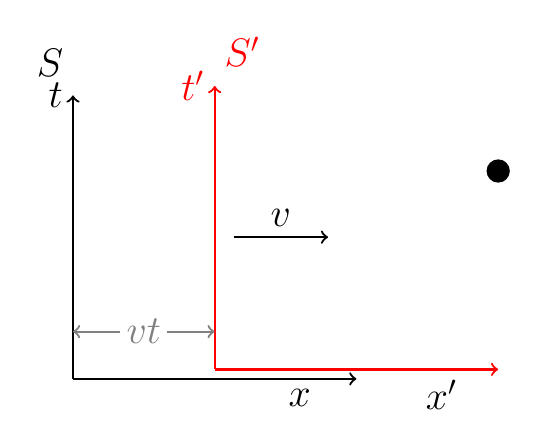
\begin{tikzpicture}[
    scale=1.2,          % Escala general de la figura
    font=\Large,        % Tamaño de la fuente para las etiquetas
    axis/.style={->, thick}, % Estilo para los ejes (flecha, grueso)
]

% --- Sistema de referencia S (estacionario, en gris) ---
% Eje horizontal x
\draw[axis, black] (0,0) -- (3,0) node[below, black, pos=0.8] {$x$};
% Eje vertical t
\draw[axis, black] (0,0) -- (0,3) node[left] {$t$};
% Etiqueta del sistema
\node[black, anchor=south east] at (0,3.1) {$S$};

% --- Sistema de referencia S' (en movimiento, en rojo) ---
% Usamos un 'scope' con 'xshift' para mover todo el sistema S'
\begin{scope}[xshift=1.5cm,yshift=0.1cm]
    % Eje horizontal x'
    \draw[axis, red] (0,0) -- (3,0) node[below, black, pos=0.8] {$x'$};
    % Eje vertical t'
    \draw[axis, red] (0,0) -- (0,3) node[left] {$t'$};
    % Etiqueta del sistema
    \node[red, anchor=south west] at (0,3.1) {$S'$};
\end{scope}

% --- Flecha de velocidad v ---
\draw[axis, black] (1.7, 1.5) -- (2.7, 1.5) node[midway, above] {$v$};

% --- Punto del evento ---
\fill[black] (4.5, 2.2) circle (3.5pt);

% --- distancia entre sistemas ---
\draw[axis, gray] (0.5, 0.5) -- (0.0, 0.5) node[midway, ,gray,pos=-0.5] {$vt$};
\draw[axis, gray] (1.0, 0.5) -- (1.5, 0.5);



\end{tikzpicture}
%\end{center}
% --- Fin del código TikZ ---
    \caption{Sistema de referencia inercial $\color{red}S'$, a velocidad constante en $x$, $v$, con respecto al sistema en reposo $S$. A un tiempo $t$ el origin de $\color{red}S'$ se encuentra a una distancia $x = vt$ del origen de $S$. }
    \label{fig:placeholder}
\end{figure}


Ahora nos enfocamos en derivar las transformaciones para $x'$ y $t'$.

\subsection{Pasos de la Derivación}

\subsubsection{Paso 1: La Suposición de Linealidad}

Las transformaciones deben ser lineales para preservar el principio de inercia. Un movimiento uniforme en un sistema debe aparecer como un movimiento uniforme en el otro. Por lo tanto, las transformaciones tienen la forma:
\begin{align}
\label{eq:tl1}
 x' = Ax + Bt\,.   
\end{align}
 
\subsubsection{Paso 2: Usando el Movimiento del Origen}

El origen de $S'$ ($x'=0$) se mueve con velocidad $v$ en el sistema $S$, por lo que su posición es $x=vt$. Sustituyendo esto en la ecuación~\eqref{eq:tl1}:
\[ 0 = A(vt) + Bt \implies B = -Av \]
Esto da $x' = A(x-vt)$. Renombramos la constante $A$ con el símbolo más convencional $\gamma$.
\begin{align}
\label{eq:xplt}
x' = \gamma (x - vt).    
\end{align}

\subsubsection{Paso 3: Aplicando el Principio de Relatividad}

La transformación inversa (de $S'$ a $S$) debe tener la misma forma, con la velocidad invertida ($v \to -v$):
\begin{align}
\label{eq:invxplt}
    x = \gamma (x' + vt').
\end{align}

\subsubsection{Paso 4: Aplicando el Segundo Postulado}
Imaginemos un pulso de luz emitido desde el origen en $t=t'=0$. Un observador en $S$ ve su frente de onda en $x=ct$, mientras que un observador en $S'$ lo ve en $x'=ct'$. Sustituyendo esto en nuestras ecuaciones de transformación:

\newcounter{paso}

\noindent
%\renewcommand{\arraystretch}{1.5}
\begin{tabular}{l|p{0.35\textwidth}|p{0.6\textwidth}}
\textbf{Paso}&\textbf{Encontrar} $\gamma$& \textbf{Paso algebraico} \\\hline
\stepcounter{paso}\thepaso)&$\begin{aligned}
    x' =& \gamma (x - vt),\\
    x = &\gamma (x' + vt').
\end{aligned}$& Ecuaciones \eqref{eq:xplt} y \eqref{eq:invxplt}\\\hline
\stepcounter{paso}\thepaso)&$\begin{aligned}[t]
ct' &= \gamma(ct - vt) = \gamma t (c-v)   \\
ct &= \gamma(ct' + vt') = \gamma t' (c+v)  
\end{aligned}$  &  Reemplazando $x=ct$ y $x'=ct'$ en  
las ecuaciones anteriores\\\hline
\stepcounter{paso}\thepaso)&$(ct')(ct) = [\gamma t (c-v)][\gamma t' (c+v)]$& Multiplicando las dos ecuaciones\\\hline
\stepcounter{paso}\thepaso)&$c^2 t' t = \gamma^2 t t' (c-v)(c+v)$& 
Realizando las operaciones indicadas\\\hline
\stepcounter{paso}\thepaso)&$c^2= \gamma^2 (c^2-v^2)$& Dividiendo por $tt'$ a ambos lados de la igualdad y expandiendo la diferencia de cuadrados \\\hline
\stepcounter{paso}\thepaso)&$1=\gamma^2(1-v^2/c^2)$&Dividiendo por $c^2$ a ambos lados de la igualdad.\\\hline
\stepcounter{paso}\thepaso)&$\gamma^2 = \dfrac{1}{1-v^2/c^2}$&
Dividiendo por $1-v^2/c^2$ a ambos lados de la igualdad.
\\[8pt]\hline
\stepcounter{paso}\thepaso)&$\gamma = \dfrac{1}{\sqrt{1-v^2/c^2}}$&
Sacando raíz cuadrada a ambos lados iguales\\[8pt]\hline
\end{tabular}

De ésta forma:
\begin{align}
\label{eq:gamma}
    \boxed{\gamma = \frac{1}{\sqrt{1 - v^2/c^2}}} \,,
\end{align}
y 
\begin{align}
\label{eq:gammasquare}
    \gamma^2 =&\frac{1}{1-\dfrac{v^2}{c^2}} =  \frac{c^2}{c^2-v^2}\,.
\end{align}

\subsubsection{Paso 6: Derivando la Transformación del Tiempo}
Dado que ya tenemos la expresión completa para $x'$, en las ecuaciones \eqref{eq:xplt} y \eqref{eq:invxplt}, podemos
despejar $t'$

\noindent
\setcounter{paso}{0}
\begin{tabular}{l|p{0.35\textwidth}|p{0.6\textwidth}}
\textbf{paso} &\textbf{Despejar} $t'$& \textbf{Paso algebraico} \\\hline
\stepcounter{paso}\thepaso) & $\begin{aligned}
    x' =& \gamma (x - vt),\\
    x = &\gamma (x' + vt').
\end{aligned}$& Ecuaciones \eqref{eq:xplt} y \eqref{eq:invxplt}\\\hline
\stepcounter{paso}\thepaso) & $x=\gamma[\gamma(x-vt) +v t']$&sustituyendo $x'=\gamma(x-vt)$ en $x = \gamma(x' + vt')$\\\hline
\stepcounter{paso}\thepaso) & $x=\gamma^2x-\gamma^2 vt +\gamma v t'$  & Distribuyendo $\gamma$ el lado derecho\\\hline
\stepcounter{paso}\thepaso) & $\gamma v t' = x-\gamma^2x +\gamma^2 v t$ & Sumando $-\gamma^2x +\gamma^2 v t$ a ambos lados de la igualdad. \\\hline
\stepcounter{paso}\thepaso) & $\gamma v t' = x(1-\gamma^2) +\gamma^2 v t$  & Factorizando $x$.\\\hline
\stepcounter{paso}\thepaso) & $\gamma v t' = x\left(1-\dfrac{c^2}{c^2-v^2}\right) +\gamma^2 v t$ & Reemplazando $\gamma^2$ de la ecuación~\eqref{eq:gammasquare} \\\hline
\stepcounter{paso}\thepaso) & $\gamma v t' = x\left(\dfrac{\cancel{c^2}-v^2-\cancel{c^2}}{c^2-v^2}\right) +\gamma^2 v t$. & Sumando las fracciones.\\\hline
\stepcounter{paso}\thepaso) & $\gamma v t' =\gamma^2 v t- xv^2\left[\dfrac{c^2}{c^2(c^2-v^2)}\right]$ & Multiplicando y dividiendo por $c^2$ en el último término. \\[5pt]\hline
\stepcounter{paso}\thepaso) & $\cancel{\gamma}\cancel{v}  t' =\gamma^{\cancel{2}}\cancel{v}  t- \gamma^{\cancel{2}} \dfrac{v^{\cancel{2}} x}{c^2}$  &
Usando de nuevo la ecuación~\eqref{eq:gammasquare} para $\gamma^2$ y cancelando términos iguales a ambos lados de la igualdad\\\hline
\stepcounter{paso}\thepaso) & $t' = \gamma\left(t-\dfrac{vx}{c^2}\right)$\\[5pt]\hline
\end{tabular}

De modo que
\[ \boxed{t' = \gamma \left( t - \frac{vx}{c^2} \right)} \]

\subsection{Resumen de las Transformaciones de Lorentz}
Las transformaciones de Lorentz completas son:
\[
\boxed{
\begin{aligned}
t' &= \gamma \left( t - \frac{vx}{c^2} \right) \\
x' &= \gamma (x - vt) \\
y' &= y \\
z' &= z
\end{aligned}
}
\]

\subsubsection{Las Transformaciones Inversas}
Las transformaciones de $S'$ a $S$ se encuentran intercambiando las coordenadas y haciendo $v \to -v$:
\[
\boxed{
\begin{aligned}
t &= \gamma \left( t' + \frac{vx'}{c^2} \right) \\
x &= \gamma (x' + vt') \\
y &= y' \\
z &= z'
\end{aligned}
}
\]

\subsubsection{Transformaciones de Galileo}
Se obtienen cuando no hay una velocidad límite, y por lo tanto $c\to \infty$
\begin{align*}
t' &= \lim_{c\to\infty}\left[\gamma \left( t - \frac{vx}{c^2} \right)\right] 
    = t\\
x' &= \lim_{c\to\infty}\left[\gamma (x - vt)\right]  = x - vt \\
y' &= y \\
z' &= z
\end{align*}

Mientras que para factor de Lorentz $\gamma$, o el factor de contracción relativista $1/\gamma$, 
\begin{align}
    \lim_{c\to\infty}\ \gamma = 1\,. 
\end{align}

Esto quiere decir que las las distancia y tiempos no están afectados por las transformaciones de Galileo.

\subsubsection{Existencia de una velocidad límite en el Universo}

Toda la evidencia experimental, desde el electromagnetismo hasta la desintegración de partículas, confirma que vivimos en un universo donde hay una velocidad límite. Llamamos a esta velocidad universal $c$, y la identificamos con la velocidad de la luz en el vacío. La constancia de la velocidad de la luz no es una suposición separada, sino una consecuencia directa de la estructura del espacio-tiempo mismo, como se demuestra en el Apendice~\ref{sec:tl}.




\section{Derivación de la Dilatación del Tiempo a partir de las Transformaciones de Lorentz}

En las aplicaciones prácticas, donde se estudia el movimiento de un cuerpo a velocidad constante, es conveniente asumir que el sistema inercial se mueve con la misma velocidad del cuerpo bajo estudio, como se ilustra en la figura~\ref{fig:movv}.

\begin{figure}
% --- Inicio del código TikZ para insertar ---
%\begin{center}
\centering
\begin{tikzpicture}[
    scale=1.2,          % Escala general de la figura
    font=\Large,        % Tamaño de la fuente para las etiquetas
    axis/.style={->, thick}, % Estilo para los ejes (flecha, grueso)
]

% --- Sistema de referencia S (estacionario, en gris) ---
% Eje horizontal x
\draw[axis, black] (0,0) -- (3,0) node[below, black, pos=0.8] {$x$};
% Eje vertical t
\draw[axis, black] (0,0) -- (0,3) node[left] {$t$};
% Etiqueta del sistema
\node[black, anchor=south east] at (0,3.1) {$S$};

% --- Sistema de referencia S' (en movimiento, en rojo) ---
% Usamos un 'scope' con 'xshift' para mover todo el sistema S'
\begin{scope}[xshift=1.5cm,yshift=0.1cm]
    % Eje horizontal x'
    \draw[axis, red] (0,0) -- (3.5,0) node[below, black, pos=0.8] {$x'$};
    % Eje vertical t'
    \draw[axis, red] (0,0) -- (0,3) node[left] {$t'$};
    % Etiqueta del sistema
    \node[red, anchor=south west] at (0,3.1) {$S'$};
\end{scope}

% --- Flecha de velocidad v ---
\draw[axis, black] (1.7, 1.5) -- (2.7, 1.5) node[midway, above] {$v$};

% --- Punto del evento ---
\fill[black] (1.7, 1.5) circle (3.5pt);

\node[inner sep=0pt] (russell) at (3.5,2)
    {
\includegraphics[scale=0.03]{clock}};

\draw[dotted] (3.5, 0.1) -- (3.5,2);

\node[black] (russell) at (3.5,-0.15) {$x'_c$};

\draw[axis, black] (3.7, 2) -- (4.7, 2) node[midway, above] {$v$};


\end{tikzpicture}
%\end{center}
% --- Fin del código TikZ ---
    \caption{Sistema de referencia inercial $\color{red}S'$, moviendos con velocidad constante en $x$, $v$, con el objeto bajo estudio }
    \label{fig:movv}
\end{figure}


La dilatación del tiempo es una consecuencia directa y famosa de las transformaciones de Lorentz. Describe el fenómeno en el que un reloj que está en movimiento relativo a un observador se mide por ese observador como si estuviera marcando el tiempo más lentamente que un reloj que está en reposo relativo a él.

Para derivar esto, estableceremos un experimento mental simple y aplicaremos la transformación de Lorentz para el tiempo.

\subsection{La Configuración Física (Experimento Mental)}

\begin{enumerate}
    \item \textbf{Dos Sistemas:} Tenemos dos sistemas inerciales, $S$ y $S'$. Como antes, el sistema $S$ es el sistema ``estacionario" (por ejemplo, un observador en el suelo), y el sistema $S'$ se mueve con una velocidad constante $v$ a lo largo del eje x relativo a $S$.

    \item \textbf{Un Reloj en el Sistema en Movimiento:} Imaginemos que hay un reloj en reposo en el sistema en movimiento, $S'$. Dado que el reloj no se mueve \textit{dentro de su propio sistema}, su posición es un valor constante, que llamaremos $x'_c$.

    \item \textbf{Dos Eventos:} Consideraremos dos eventos, que son dos "tictacs" consecutivos de este reloj.
    \begin{itemize}
        \item \textbf{Evento 1:} El reloj hace tictac por primera vez. Desde la perspectiva de un observador en el sistema $S'$, este evento ocurre en las coordenadas $(t'_1, x'_c)$.
        \item \textbf{Evento 2:} El reloj hace tictac por segunda vez. En el sistema $S'$, este evento ocurre en las coordenadas $(t'_2, x'_c)$.
    \end{itemize}
\end{enumerate}

\subsection{Definiendo el Tiempo Propio}

El intervalo de tiempo entre dos eventos que ocurren en la \textbf{misma ubicación espacial} en un sistema dado se llama \textbf{intervalo de tiempo propio}, denotado por $\Delta t_0$.

En nuestra configuración, los dos tictacs del reloj ocurren en la misma ubicación ($x'_c$) en el sistema $S'$. Por lo tanto, el intervalo de tiempo medido por un observador en el sistema en movimiento $S'$ es el tiempo propio:
\[ \Delta t_0 = t'_2 - t'_1 \]
Nuestro objetivo es encontrar el intervalo de tiempo entre estos mismos dos eventos según lo medido por el observador en el sistema estacionario $S$. Llamemos a este intervalo $\Delta t$.
\[ \Delta t = t_2 - t_1 \]

\subsection{Aplicando las Transformaciones de Lorentz}

Necesitamos relacionar las coordenadas de tiempo en $S$ con las coordenadas en $S'$. La transformación de Lorentz inversa para el tiempo es la opción más conveniente aquí, ya que expresa el tiempo del sistema estacionario ($t$) en términos de las coordenadas del sistema en movimiento ($t', x'$).
\[ t = \gamma \left( t' + \frac{vx'}{c^2} \right) \]
Ahora, aplicamos esta transformación a nuestros dos eventos:
\begin{enumerate}
    \item El tiempo del Evento 1 medido en el sistema $S$ es $t_1$:
    \[ t_1 = \gamma \left( t'_1 + \frac{vx'_c}{c^2} \right) \]
    \item El tiempo del Evento 2 medido en el sistema $S$ es $t_2$:
    \[ t_2 = \gamma \left( t'_2 + \frac{vx'_c}{c^2} \right) \]
\end{enumerate}

\subsection{La Derivación}

El intervalo de tiempo $\Delta t$ medido por el observador en el sistema $S$ es la diferencia entre $t_2$ y $t_1$.
\begin{align*}
\Delta t &= t_2 - t_1 \\
&= \left[ \gamma \left( t'_2 + \frac{vx'_c}{c^2} \right) \right] - \left[ \gamma \left( t'_1 + \frac{vx'_c}{c^2} \right) \right] \\
&= \gamma \left( t'_2 + \frac{vx'_c}{c^2} - t'_1 - \frac{vx'_c}{c^2} \right) \\
&= \gamma (t'_2 - t'_1)
\end{align*}
El término que involucra la posición $x'_c$ se cancela precisamente porque el reloj estaba en reposo en el sistema $S'$. Ahora sustituimos la definición de tiempo propio, $\Delta t_0 = t'_2 - t'_1$:
\[ \Delta t = \gamma \Delta t_0 \]

\subsection{Resultado e Interpretación}

La fórmula final para la dilatación del tiempo se obtiene sustituyendo la expresión para $\gamma$:
\[ \boxed{ \Delta t = \frac{\Delta t_0}{\sqrt{1 - v^2/c^2}} } \]
Interpretemos este importante resultado:
\begin{itemize}
    \item El factor de Lorentz $\gamma = \frac{1}{\sqrt{1 - v^2/c^2}}$ es siempre mayor o igual a 1, ya que la velocidad $v$ debe ser menor que $c$.
    \item Esto significa que $\Delta t \ge \Delta t_0$.
    \item El intervalo de tiempo ($\Delta t$) medido por el observador en el sistema ``estacionario" $S$ es \textit{más largo} que el intervalo de tiempo propio ($\Delta t_0$) medido en el sistema de reposo del reloj.
\end{itemize}
Un intervalo de tiempo más largo entre tictacs significa que se observa que el reloj funciona más lentamente. Por lo tanto, el observador en $S$ concluye que el reloj en movimiento funciona lentamente en comparación con su propio reloj idéntico. Este fenómeno es la \textbf{dilatación del tiempo}.


\section{Derivación de la Contracción de la Longitud a partir de las Transformaciones de Lorentz}

\begin{figure}
% --- Inicio del código TikZ para insertar ---
%\begin{center}
\centering
\begin{tikzpicture}[
    scale=1.2,          % Escala general de la figura
    font=\Large,        % Tamaño de la fuente para las etiquetas
    axis/.style={->, thick}, % Estilo para los ejes (flecha, grueso)
]

% --- Sistema de referencia S (estacionario, en gris) ---
% Eje horizontal x
\draw[axis, black] (0,0) -- (4,0) node[below, black, pos=0.5] {$x$};
% Eje vertical t
\draw[axis, black] (0,0) -- (0,3) node[left] {$t$};
% Etiqueta del sistema
\node[black, anchor=south east] at (0,3.1) {$S$};

% --- Sistema de referencia S' (en movimiento, en rojo) ---
% Usamos un 'scope' con 'xshift' para mover todo el sistema S'
\begin{scope}[xshift=1.5cm,yshift=0.1cm]
    % Eje horizontal x'
    \draw[axis, red] (0,0) -- (3.5,0) node[below, black, pos=0.8] {$x'$};
    % Eje vertical t'
    \draw[axis, red] (0,0) -- (0,3) node[left] {$t'$};
    % Etiqueta del sistema
    \node[red, anchor=south west] at (0,3.1) {$S'$};
\end{scope}

% --- Flecha de velocidad v ---
\draw[axis, black] (1.7, 1.5) -- (2.7, 1.5) node[midway, above] {$v$};

% --- Punto del evento ---
\fill[black] (1.7, 1.5) circle (3.5pt);

\node[inner sep=0pt] (russell) at (3.32,2)
    {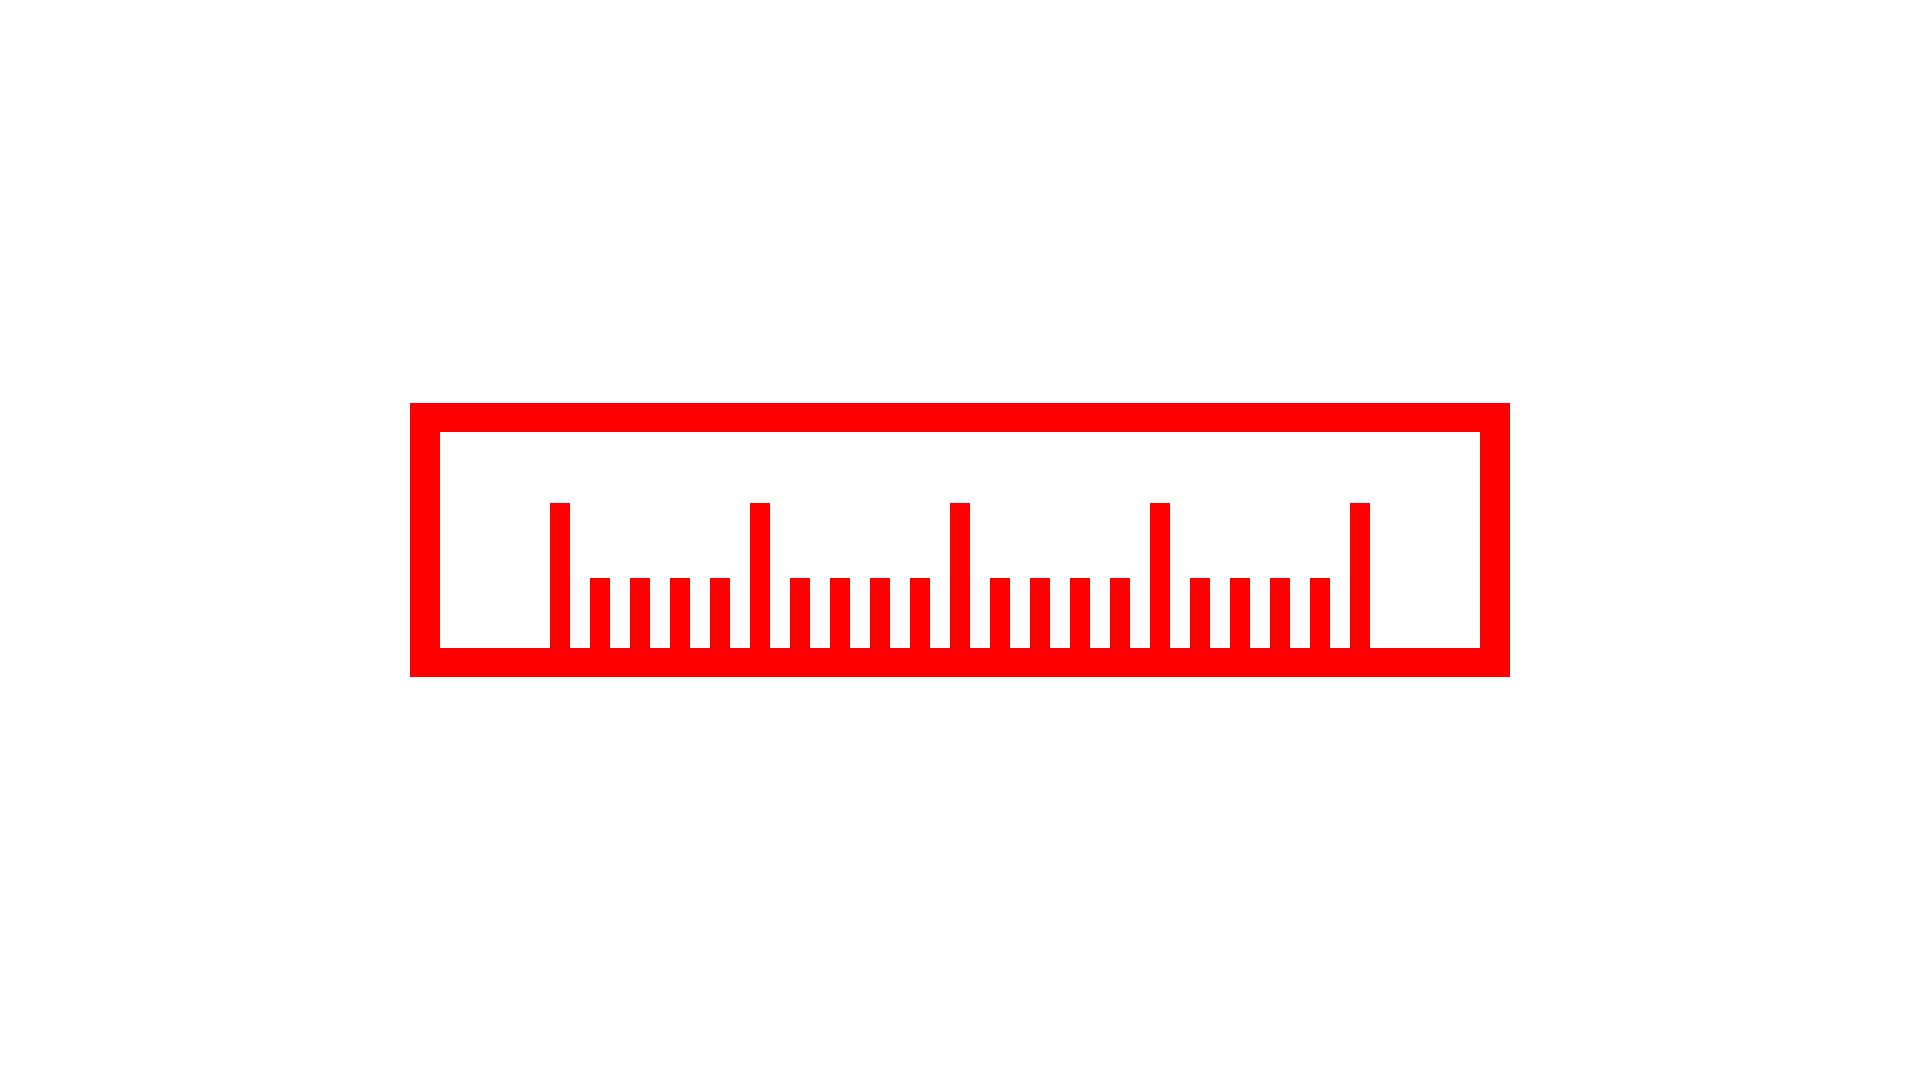
\includegraphics[scale=0.1]{ruler}};


\draw[dotted] (2.95, -0.2) -- (2.95,2);
\node[black] (russell) at (2.95,-0.2) {$x_1$};

\draw[dotted] (3.7, -0.2) -- (3.7,2);
\node[black] (russell) at (3.7,-0.2) {$x_2$};


%\draw[axis, black] (3.7, 2) -- (4.7, 2) node[midway, above] {$v$};

% --- distancia entre sistemas ---
\draw[axis, gray] (3.15, 0.5) -- (2.95, 0.5) node[midway, ,gray,pos=-0.8] {$t$};
\draw[axis, gray] (3.5, 0.5) -- (3.7, 0.5);



\end{tikzpicture}
%\end{center}
% --- Fin del código TikZ ---
    \caption{Sistema de referencia inercial $\color{red}S'$, moviendos con velocidad constante en $x$, $v$, con el objeto bajo estudio }
    \label{fig:movruler}
\end{figure}




La contracción de la longitud es otra predicción fundamental de la Relatividad Especial. Afirma que se mide que un objeto en movimiento es más corto a lo largo de su dirección de movimiento que su longitud cuando se mide en reposo. Este efecto también se conoce como contracción de Lorentz.

La clave para medir correctamente la longitud de un objeto en movimiento es determinar las posiciones de sus dos extremos \textbf{simultáneamente} en el sistema de referencia del observador.

La longitud propia, $L_0$, es la distancia entre dos puntos cuyas posiciones son medidas por un observador en reposo respecto a los dos puntos. La longitud contraida se denota como $L_0$

% --- Inicio del código LaTeX para insertar ---

\section*{Demostración de la Contracción de Lorentz a partir de la Dilatación del Tiempo}

Esta es una de las demostraciones más elegantes en relatividad, ya que muestra cuán profundamente entrelazados están el espacio y el tiempo. En lugar de derivar la contracción de la longitud directamente de los postulados, la derivaremos como una consecuencia lógica de la dilatación del tiempo. Para ello, construiremos un experimento mental que involucre tanto una medición de distancia como una de tiempo desde dos perspectivas diferentes.

\subsection*{El Experimento Mental}
Imaginemos un viaje espacial:
\begin{itemize}
    \item Hay dos puntos fijos en el espacio: un punto de partida (la Tierra) y un punto de destino (una estrella lejana).
    \item Un observador en la Tierra (en el sistema de referencia \textbf{S}) mide la distancia entre la Tierra y la estrella. Como esta distancia está en reposo con respecto a él, mide la \textbf{longitud propia}, $L_0$.
    \item Una nave espacial (en el sistema de referencia \textbf{S'}) viaja de la Tierra a la estrella a una velocidad constante $v$.
\end{itemize}
Nuestro objetivo es encontrar la distancia entre la Tierra y la estrella medida por el astronauta en la nave, a la que llamaremos $L$.

\subsection*{La Demostración: Paso a Paso}
La demostración se basa en calcular el tiempo del viaje desde ambas perspectivas y luego conectarlos usando la fórmula de la dilatación del tiempo.

\subsubsection*{Paso 1: La Perspectiva de la Tierra (Sistema S)}
\begin{itemize}
    \item \textbf{Distancia del viaje:} Para el observador en la Tierra, la distancia que debe recorrer la nave es la longitud propia, $L_0$.
    \item \textbf{Tiempo del viaje:} El observador en la Tierra mide el tiempo que tarda la nave en completar el viaje usando sus propios relojes. Llamaremos a este tiempo $\Delta t$. Usando la fórmula básica \texttt{tiempo = distancia / velocidad}, tenemos:
    \[ \Delta t = \frac{L_0}{v} \]
\end{itemize}
Despejando la distancia, obtenemos nuestra primera ecuación clave:
\begin{equation} \label{eq:dist_tierra}
    L_0 = v \cdot \Delta t
\end{equation}

\subsubsection*{Paso 2: La Perspectiva del Astronauta (Sistema S')}
\begin{itemize}
    \item \textbf{Distancia del viaje:} Para el astronauta, él está en reposo y es la estrella la que se acerca a él a una velocidad $v$. La distancia que él mide entre la Tierra y la estrella es $L$.
    \item \textbf{Tiempo del viaje:} El astronauta mide la duración del viaje en su propio reloj. Este tiempo es el \textbf{tiempo propio}, $\Delta t_0$, porque para él, los eventos de ``salida" y ``llegada" ocurren en su misma ubicación (en $x'=0$). De nuevo, usando \texttt{tiempo = distancia / velocidad}:
    \[ \Delta t_0 = \frac{L}{v} \]
\end{itemize}
Despejando la distancia, obtenemos nuestra segunda ecuación clave:
\begin{equation} \label{eq:dist_nave}
    L = v \cdot \Delta t_0
\end{equation}

\subsubsection*{Paso 3: El Puente - Conectando las Perspectivas con la Dilatación del Tiempo}
Ahora tenemos dos ecuaciones diferentes para la distancia, cada una involucrando una medida de tiempo diferente. Aquí es donde entra en juego la \textbf{dilatación del tiempo}, que actúa como un puente entre los dos sistemas de referencia.

La fórmula de la dilatación del tiempo nos dice cómo se relacionan el tiempo medido por el observador en la Tierra ($\Delta t$) y el tiempo propio medido por el astronauta ($\Delta t_0$):
\begin{equation} \label{eq:dilatacion}
    \Delta t = \gamma \Delta t_0 \quad \text{donde} \quad \gamma = \frac{1}{\sqrt{1 - v^2/c^2}}
\end{equation}

\subsubsection*{Paso 4: Combinar las Ecuaciones y Resolver}
Tenemos un sistema de tres ecuaciones y nuestro objetivo es encontrar una relación entre $L$ y $L_0$.
\begin{enumerate}
    \item Partimos de la Ecuación (\ref{eq:dist_tierra}):
    \[ L_0 = v \cdot \Delta t \]
    \item Sustituimos la Ecuación (\ref{eq:dilatacion}) en la ecuación anterior para eliminar $\Delta t$:
    \[ L_0 = v \cdot (\gamma \Delta t_0) \]
    \item Ahora, observamos la Ecuación (\ref{eq:dist_nave}), que nos dice que $L = v \cdot \Delta t_0$. Podemos sustituir todo el término $(v \cdot \Delta t_0)$ en nuestra ecuación actual por $L$:
    \[ L_0 = \gamma (v \cdot \Delta t_0) \implies L_0 = \gamma L \]
\end{enumerate}
Finalmente, despejamos $L$, la longitud medida por el astronauta en movimiento:
\[ L = \frac{L_0}{\gamma} \]

\subsection*{Resultado y Conclusión}
Al sustituir la expresión completa para $\gamma$, obtenemos la fórmula de la contracción de la longitud:
\[ \boxed{ L = L_0 \sqrt{1 - v^2/c^2} } \]
Hemos demostrado con éxito que la contracción de la longitud es una consecuencia directa y necesaria de la dilatación del tiempo. Al insistir en que ambos observadores deben estar de acuerdo en los hechos básicos, inevitablemente llegamos a la conclusión de que para el objeto en movimiento la distancia del viaje es más corta. Esto subraya que el espacio y el tiempo están intrínsecamente entrelazados.

% --- Fin del código LaTeX ---

ver \url{https://inspirehep.net/literature/2825885}


\section{Suma de velocidades relativista}

En la física clásica (galileana), si estás en un tren que se mueve a una velocidad $v$, y lanzas una pelota hacia adelante a una velocidad $u'$ (relativa al tren), un observador en el suelo vería la pelota moverse a una simple suma de las velocidades:
\[ u = u' + v \quad \text{(Suma Clásica/Galileana)} \]
Esto funciona perfectamente a velocidades cotidianas. Sin embargo, se rompe a velocidades relativistas.

\textbf{La Contradicción:} Imagina una nave espacial (sistema $S'$) que se aleja de la Tierra (sistema $S$) a $v=0.8c$. La nave dispara una sonda hacia adelante a una velocidad de $u'=0.7c$ relativa a sí misma. Según la fórmula clásica, un observador en la Tierra vería la sonda moverse a:
\[ u = 0.7c + 0.8c = 1.5c \]
Esto es más rápido que la velocidad de la luz, lo cual viola el segundo postulado de la Relatividad Especial. Necesitamos una nueva fórmula que respete el límite de velocidad cósmico.

\subsection{La Configuración para la Fórmula Relativista}

Usamos tres sistemas de referencia:
\begin{itemize}
    \item \textbf{Sistema S:} Un observador estacionario (por ejemplo, en la Tierra).
    \item \textbf{Sistema S':} Un sistema que se mueve con velocidad $v$ relativa a $S$ (por ejemplo, la nave espacial).
    \item \textbf{Objeto:} Un objeto que se mueve con velocidad $u'$ relativa a $S'$.
\end{itemize}
Nuestro objetivo es encontrar la velocidad del objeto, \textbf{$u$}, medida por el observador en el sistema estacionario, $S$.
\[
\text{S (Tierra)} \quad \xrightarrow{v} \quad \text{S' (Nave)} \quad \xrightarrow{u'} \quad \text{Objeto (Sonda)}
\]
\[
\text{¿Cuál es la velocidad } u \text{ del Objeto relativa a S?}
\]

\subsection{Derivación a partir de las Transformaciones de Lorentz}

Las velocidades constantes se definen como el cociente entre la posición y el tiempo:
\[ u = \frac{x}{t} \quad \text{y} \quad u' = \frac{x'}{t'}\,, \]
que son respectivamente las velocidades del un objeto con respecto a los sistemas $S$ y $S'$ que se me mueve a su vez con una velocidad $v$

Comenzamos con las transformaciones de Lorentz que relacionan las coordenadas:
\begin{align*}
x' &= \gamma(x - vt) \\
t' &= \gamma\left(t - \frac{vx}{c^2}\right)
\end{align*}
Ahora, podemos construir la fracción para $u'$ dividiendo $x'$ por $t'$:
\[ u' = \frac{x'}{t'} = \frac{\gamma(x - vt)}{\gamma\left(t - \frac{v\,x}{c^2}\right)} \]
Los factores $\gamma$ se cancelan:
\[ u' = \frac{x - v\,t}{t - \frac{v\,x}{c^2}} \]
Para poner esto en términos de velocidades, dividimos el numerador y el denominador por $dt$:
\[ u' = \frac{\frac{x}{t} - v\frac{t}{t}}{\frac{t}{t} - \frac{v}{c^2}\frac{x}{t}} \]
Sustituyendo $u = \frac{x}{t}$:
\[ u' = \frac{u - v}{1 - \frac{uv}{c^2}} \]
Esta fórmula da la velocidad relativa $u'$ cuando conoces las velocidades en el sistema estacionario. Sin embargo, queremos ``sumar" velocidades, lo que significa que necesitamos resolver esta ecuación para $u$.

\noindent
\setcounter{paso}{0}
\begin{tabular}{l|p{0.35\textwidth}|p{0.6\textwidth}}
\textbf{paso} &\textbf{Despejar} $u$& \textbf{Paso algebraico} \\\hline
\stepcounter{paso}\thepaso) & $ u' = \dfrac{u - v}{1 - \frac{uv}{c^2}} $
 & Ecuación inicial \\[5pt]\hline
\stepcounter{paso}\thepaso) & $u'\left(1 - \dfrac{uv}{c^2}\right) = u - v $ & Multiplicar por $\left(1 - \dfrac{uv}{c^2}\right)$ a ambos lados de la igualdad \\[5pt]\hline
\stepcounter{paso}\thepaso) & $u' - \dfrac{u'uv}{c^2} = u - v$ & Distribuir $u'$ en el lado derecho.\\[5pt]\hline
\stepcounter{paso}\thepaso) & $u' + v = u + \dfrac{u'uv}{c^2}$ & Reunir términos con $u$. \\[5pt]\hline
\stepcounter{paso}\thepaso) & $u' + v = u\left(1 + \dfrac{u'v}{c^2}\right)$ & Factorizar $u$. \\[5pt]\hline
\stepcounter{paso}\thepaso) & $u = \dfrac{u' + v}{1 + \frac{u'v}{c^2}}$& Dividiendo por $\left(1 + \dfrac{u'v}{c^2}\right)$ a ambos lados de la igualdad.\\[7pt]\hline

\end{tabular}


De esta forma obtenemos da la \textbf{Fórmula de Suma de Velocidades de Einstein}:
\[
\boxed{
u = \frac{u' + v}{1 + \frac{u'v}{c^2}}
}
\]

\subsection*{Ejercicio: Despejar $c^2$ de la fórmula de suma de velocidades}
\noindent
\setcounter{paso}{0}
\begin{tabular}{l|p{0.3\textwidth}|p{0.65\textwidth}}
\textbf{paso} &\textbf{Despejar} $c^2$& \textbf{Paso algebraico} \\\hline
\stepcounter{paso}\thepaso) & $u = \dfrac{u' + v}{1 + \frac{u'v}{c^2}}$& Ecuación inicial\\[7pt]\hline
\stepcounter{paso}\thepaso) & $u\left(1 + \dfrac{u'v}{c^2}\right) = u' + v $ & Multiplicar por $\left(1 + \dfrac{u'v}{c^2}\right)$ a ambos lados de la igualdad. \\[5pt]\hline
\stepcounter{paso}\thepaso) & \phantom{$u + \dfrac{u u'v}{c^2} =  u' + v$}& Distribuir $u$ en el lado derecho.\\[5pt]\hline
\stepcounter{paso}\thepaso) & $\dfrac{u u'v}{c^2} =  u' + v - u$& \phantom{Restar $u$ a ambos lados de la igualdad.}\\[5pt]\hline
\stepcounter{paso}\thepaso) &\phantom{ $\dfrac{c^2}{u u'v} = \dfrac{1}{ u' + v - u}$}& Tomar el reciproco a ambos lados de la igualdad.\\[5pt]\hline
\stepcounter{paso}\thepaso) & $c^2 = \dfrac{u u'v}{ u' + v - u}$ & \phantom{ Multiplicar por $u u'v$ a ambos lados de la igualdad. }\\[5pt]\hline
\end{tabular}

El resultado de despejar $c^2$ es entonces

\begin{align}
\boxed{
    c^2 = \dfrac{u u'v}{ u' + v - u}
    \,.}
\end{align}

En el límite no relativista de $u\approx u'+v$, tenemos que
\begin{align}
    c^2 = \dfrac{u u'v}{ u' + v - u} \approx \dfrac{(u'+v) u'v}{0} = \infty\,, 
\end{align}
tenemos que  $c = \infty$ y de éste modo en el límite no relativista, ¡no existe una velocidad límite!.


\subsection{Características Clave y Ejemplos}

\subsubsection{Ejemplo 1: La Nave Espacial y la Sonda}
Volvamos a nuestro problema inicial con la fórmula relativista.
\begin{itemize}
    \item $v = 0.8c$ (velocidad de la nave relativa a la Tierra)
    \item $u' = 0.7c$ (velocidad de la sonda relativa a la nave)
\end{itemize}
\[ u = \frac{0.7c + 0.8c}{1 + \frac{(0.7c)(0.8c)}{c^2}} = \frac{1.5c}{1 + \frac{0.56c^2}{c^2}} = \frac{1.5c}{1 + 0.56} = \frac{1.5c}{1.56} \]
\[ u \approx 0.9615c \]
El resultado es menor que la velocidad de la luz, como se requiere.

\subsubsection{Característica 1: La Velocidad de la Luz es el Límite Último}
¿Qué pasa si la nave que se mueve a $v=0.9c$ dispara un rayo láser hacia adelante ($u'=c$)?
\[ u = \frac{c + 0.9c}{1 + \frac{(c)(0.9c)}{c^2}} = \frac{1.9c}{1 + 0.9} = \frac{1.9c}{1.9} = c \]
El observador en la Tierra también mide la velocidad del rayo láser como exactamente $c$. Este hermoso resultado muestra cómo la fórmula defiende perfectamente el segundo postulado de la relatividad. 

\subsubsection{Característica 2: Se Reduce a la Fórmula Clásica a Bajas Velocidades}
Si $v \ll c$ y $u' \ll c$, el término $\frac{u'v}{c^2}$ se vuelve extremadamente pequeño y se aproxima a cero.
\[ u = \frac{u' + v}{1 + \frac{u'v}{c^2}} \approx \frac{u' + v}{1} = u' + v \]
Esto muestra que la fórmula relativista contiene la fórmula clásica como una aproximación a baja velocidad, lo cual es un requisito clave para cualquier nueva teoría física.

% --- Inicio del código LaTeX para insertar ---

\section{Fórmulas del Decaimiento Radiactivo}
En esta sección estableceremos el concepto de vida media para una partícula inestable y veremos como la relatividad especial puede afectar el tiempo de vida media dependiendo del observador inercial
\subsection*{Introducción: La Naturaleza del Decaimiento}

El decaimiento de una partícula inestable (ya sea un núcleo atómico o una partícula subatómica) es un proceso fundamentalmente \textbf{probabilístico y aleatorio}. No podemos predecir cuándo decaerá una partícula específica. Sin embargo, para una población grande de partículas idénticas, podemos predecir con gran precisión cuántas de ellas decaerán en un intervalo de tiempo determinado.

El principio clave es que la tasa de decaimiento (el número de partículas que decaen por segundo) es directamente proporcional al número de partículas que aún no han decaído. Esto conduce a una ley de \textbf{decaimiento exponencial}.

\subsection*{Fórmula 1: En Términos de la Constante de Decaimiento ($\lambda$)}

Esta es la forma más fundamental de la ecuación, derivada directamente del principio de proporcionalidad. La tasa de cambio del número de partículas, $N$, con respecto al tiempo, $t$, es:
\[ \frac{dN}{dt} = -\lambda N \]
Donde $\lambda$ (lambda) es la \textbf{constante de decaimiento} y representa la probabilidad de que una sola partícula decaiga por unidad de tiempo. Resolviendo esta ecuación diferencial, obtenemos la \textbf{fórmula del decaimiento exponencial}:
\[ \boxed{N(t) = N_0 e^{-\lambda t}} \]
Donde:
\begin{itemize}
    \item $N(t)$ es el número de partículas que quedan en el tiempo $t$.
    \item $N_0$ es el número inicial de partículas en el tiempo $t=0$.
    \item $e$ es la base del logaritmo natural.
    \item $\lambda$ es la constante de decaimiento, con unidades de (tiempo)\textsuperscript{-1} (p. ej., \si{\per\second}).
\end{itemize}

\subsection*{Fórmula 2: En Términos de la Vida Media ($t_{1/2}$)}

Esta forma es más intuitiva. La \textbf{vida media ($t_{1/2}$)} es el tiempo que tarda en decaer la mitad de una muestra inicial de partículas.

\subsubsection*{Relación entre $\lambda$ y $t_{1/2}$}
Podemos encontrar esta relación usando la primera fórmula. Por definición, cuando $t = t_{1/2}$, el número de partículas restantes es $N(t_{1/2}) = N_0/2$.
\[ \frac{N_0}{2} = N_0 e^{-\lambda t_{1/2}} \implies \frac{1}{2} = e^{-\lambda t_{1/2}} \]
Tomando el logaritmo natural de ambos lados:
\[ \ln\left(\frac{1}{2}\right) = -\lambda t_{1/2} \implies -\ln(2) = -\lambda t_{1/2} \]
Esto nos da la relación fundamental:
\[ \boxed{\lambda = \frac{\ln(2)}{t_{1/2}}} \]
Sustituyendo esta expresión para $\lambda$ en la primera fórmula de decaimiento:
\[ N(t) = N_0 e^{-\left(\frac{\ln(2)}{t_{1/2}}\right)t} = N_0 \left(e^{\ln(2)}\right)^{-\frac{t}{t_{1/2}}} = N_0 (2)^{-\frac{t}{t_{1/2}}} \]
Esto nos da la \textbf{fórmula del decaimiento en términos de la vida media}:
\[ \boxed{N(t) = N_0 \left(\frac{1}{2}\right)^{\frac{t}{t_{1/2}}}} \]
Esta forma es muy fácil de interpretar: el exponente ${t}/{t_{1/2}}$ simplemente cuenta ``cuántas vidas medias han pasado'', ver figura~\ref{fig:decrad}.

\begin{figure}
    \centering
    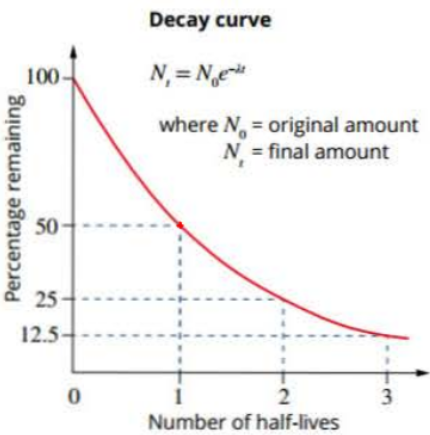
\includegraphics[width=0.4\linewidth]{decaimiento}
    \caption{Decaimiento radiativo. Tomado de \cite{} }
    \label{fig:decrad}
\end{figure}

\subsection*{Ejemplos Aplicados}
Aquí aplicamos las fórmulas a tres ejemplos que abarcan escalas de tiempo drásticamente diferentes.

\begin{table}[h!]
\centering
\caption{Comparación de Vidas Medias y Constantes de Decaimiento.}
\label{tab:decay_examples}
\begin{tabular}{l | l | p{2.7cm} | p{5.5cm}}
\hline
\textbf{Partícula} & \textbf{Vida Media ($t_{1/2}$)} & \textbf{C. de Decaimiento ($\lambda$)} & \textbf{Contexto Físico} \\
\hline \hline
Uranio-238 & \SI{4.47e9}{years} & \SI{4.91e-18}{\per\second} & Isótopo extremadamente estable, clave para la datación radiométrica de rocas muy antiguas y la edad de la Tierra. \\
\hline
Neutrón (libre) & \SI{877}{\second} (\SI{14.6}{min}) & \SI{7.9e-4}{\per\second} & Estable dentro de un núcleo, pero inestable cuando está libre. Su vida media es crucial en la cosmología del universo temprano. \\
\hline
Muón & \SI{2.2}{\micro\second} (\SI{2.2e-6}{\second}) & \SI{3.15e5}{\per\second} & Partícula fundamental muy inestable. Su detección en la superficie terrestre es una prueba experimental clásica de la dilatación del tiempo. \\
\hline
\end{tabular}
\end{table}

\paragraph{Cálculos de $\lambda$:}
\begin{itemize}
    \item \textbf{Uranio-238:}
    \begin{itemize}
        \item $t_{1/2} = \SI{4.47e9}{años} \times \SI{3.15e7}{\second\per\text{año}} \approx \SI{1.41e17}{\second}$
        \item $\lambda = \frac{\ln(2)}{\SI{1.41e17}{\second}} \approx \SI{4.91e-18}{\per\second}$
    \end{itemize}
    \item \textbf{Neutrón:}
    \[ \lambda = \frac{\ln(2)}{\SI{877}{\second}} \approx \SI{7.9e-4}{\per\second} \]
    \item \textbf{Muón:}
    \[ \lambda = \frac{\ln(2)}{\SI{2.2e-6}{\second}} \approx \SI{3.15e5}{\per\second} \]
\end{itemize}

% --- Fin del código LaTeX ---



\section{Ejemplos}
\begin{enumerate}
\item Supongamos que un cañón de bolas de tenis es capaz de lanzar una bola de tenis, de diámetro $d = \qty{67}{\milli\m}$  a la mitad de la velocidad de la luz hacia la raqueta de un tenista al otro lado de una cancha de longitud $h=\qty{24}{\m}$. Una hormiga accidentalmente resultó viajando con la bola. Calcular el tiempo propio que siente la hormiga y el tiempo dilatado para el tenista. Calcular las distancias contraídas con respecto a cada observador (ver figura \ref{fig:dilcon}). 

\begin{figure}
    \centering
    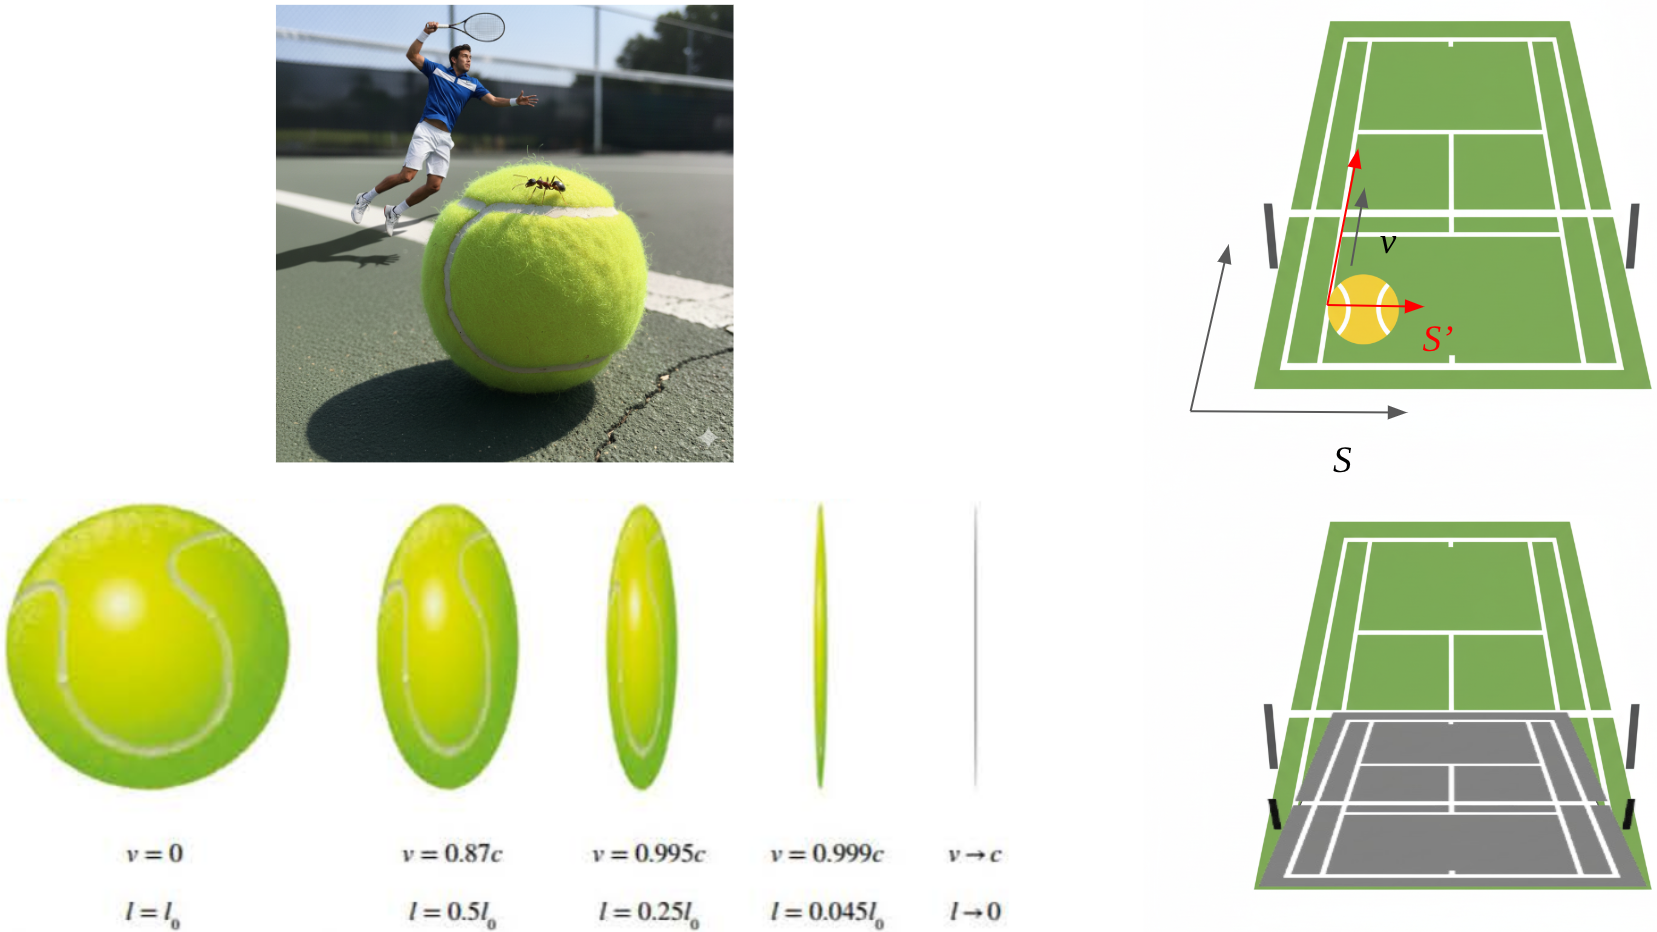
\includegraphics[width=1\linewidth]{tennis.png}
    \caption{Dilatación y contracción en un ejemplo ficticio para una bola de tenis a velocidades relativistas. En la parte de inferior se ilustra de contracción de las longitudes para la bola observada por el tenista, y la contracción de la cancha, en gris, percibida por la hormiga moviendose con la bola de tenis a una velocidad de $0.87c$ correspondiente a una contracción de Lorentz por un factor de $0.5$.}
    \label{fig:dilcon}
\end{figure}

\subsection*{Solución}
Tenemos que
\begin{itemize}
\item Escogemos el sistema $S$ con origen en el tenista
\item  Esogemos el sistema $S'$ viajando con la bola de tenis.
\item $v = 0.87c$ es la velocidad de la bola con respecto a $S$.
\item Longitud de la cancha de tenis: $h = \qty{24}{m}$ 
\item Diámetro pelota de tenis:  $d = \qty{67}{\milli\m}$
\end{itemize}

El tiempo que tarda la pelota en atravesar la cancha con respecto al tenista es el tiempo dilatado
\begin{align}
    \Delta t = \frac{h}{v} = \frac{\qty{24}{\m}}{0.87\cdot \qty{3e8}{\m/\s}} = \qty{9.2e-8}{\s}\,.
\end{align}

El tiempo que percibe la hormiga es el tiempo propio
\begin{align}
    \Delta t_0 = \frac{\Delta t}{\gamma} =& \Delta t \sqrt{1-v^2/c^2} \nonumber\\
    =& \qty{9.2e-8}{\s} \sqrt{1-0.87^2} \nonumber\\
 \approx &0.5\cdot \qty{9.2e-8}{\s} \nonumber\\
    =& \qty{4.6e-8}{\s}
\end{align}

Para calcular las distancias con respecto al tenista, partimos del hecho que su distancia propia:
\begin{quote}
    La distancia entre dos puntos cuyas posiciones son medidas por
un observador en reposo respecto a los dos puntos,
\end{quote}
corresponde a 
\begin{align*}
    L_0^{c} = h = \qty{24}{m}\,.
\end{align*}
El tenista observa la bola de diámetro propio percibido por la hormiga $L^b_0 = d$, con un diámetro contraído, como se muestra en la parte inferior de la figura~\ref{fig:dilcon}
\begin{align*}
    L^b = \frac{L^b_0}{\gamma} =& d \sqrt{1-v^2/c^2} \\
        =& d\sqrt{1-0.87^2}\\
        \approx& 0.5d\\
    =& 0.5\cdot \qty{67}{\milli\m}\\
    =& \qty{33.5}{\milli\m}\,.
\end{align*}

Finalmente, para las distancias percibidas por la hormiga, partimos del hecho para ella la bola está en su distancia propia $L^b_0 = d$.

Sin embargo, percibe una distancia de la cancha de tenis contraída, dada por
\begin{align*}
    L^{b} = \frac{L^b_0}{\gamma} =& h\sqrt{1-v^2/c^2}\\
    \approx& 0.5 h\\
        =& 0.5\cdot \qty{24}{\m}\\
    =& \qty{12}{\m}\,.
\end{align*}

Podemos de hecho comprobar que en su tiempo propio, $\Delta t_0 = \qty{4.6e-8}{s}$, que es más corto que el tiempo dilatado $\Delta t$, puede recorrer esa distancia contraída con $v=0.87c$
\begin{align*}
    L^{b} = &v \Delta t_0 \\
    =&0.87 c \cdot \qty{4.6e-8}{s}\\
    =&\qty{12}{ m }.
\end{align*}

    
 \item La estrella Xquar está a una distancia de 5 años luz de la
Tierra. La aventurera espacial Raqu se dirige desde la Tierra
hacia Xquar a una velocidad de $0.9c$.
\begin{enumerate}[label=(\alph*)]
    \item Para aquellos que observan desde la Tierra, ¿cuánto tiempo tardará
Raqu en llegar a Xquar?
\item Desde el punto de vista de Raqu, ¿cuánto tiempo tardará ella
en llegar a Xquar?
\item Aunque Xquar estaba a 5 años luz de la Tierra
y Raqu viajó a 0.9c, su viaje tomó mucho
menos tiempo de lo que se podría esperar de estas cifras.
Explique por qué es esto.
\end{enumerate}


\item Un muón es creado en la atmósfera a 15~Km de altura. Viaja hacia el centro de la Tierra a una velocidad de $0.999c$. 
\label{item:muon}

\begin{enumerate}[label=(\alph*)]
    \item Para aquellos que observan desde la Tierra, ¿cuánto tiempo tardará
el muón en llegar a la superficie de la Tierra?
\item Desde el punto de vista del muón, ¿cuánto tiempo tardará
en llegar a la superficie de la Tierra?
\item Aunque la distancia recorrida fue de 15km hasta la superficie de la Tierra y el muón viajó a $0.999c$, 
su viaje tomó mucho
menos tiempo de lo que se podría esperar de estas cifras.
Explique por qué es esto. ¿Es consistente con la vida media del muón?
\end{enumerate}

\section*{Soluciones}

\begin{itemize}
    \item[\ref{item:muon}.]

\textbf{(a) Para aquellos que observan desde la Tierra, ¿cuánto tiempo tardará el muón en llegar a la superficie de la Tierra?}

Esto se pregunta desde la perspectiva del observador "estacionario" en la Tierra. El cálculo se basa en la distancia y la velocidad medidas en el sistema de la Tierra.

\begin{itemize}
    \item \textbf{Distancia a recorrer ($L_0$):} 15 km = 15,000 m
    \item \textbf{Velocidad de viaje ($v$):} 0.999c
    \item \textbf{Velocidad de la luz ($c$):} Aproximadamente $3 \times 10^8$ m/s
\end{itemize}
Usamos la fórmula estándar para el tiempo:
\[ \text{Tiempo} = \frac{\text{Distancia}}{\text{Velocidad}} \]
\[ \Delta t = \frac{15,000 \text{ m}}{0.999 \times (3 \times 10^8 \text{ m/s})} = \frac{15,000}{2.997 \times 10^8} \text{ s} \approx 5.005 \times 10^{-5} \text{ s} \]
Para hacer este número más intuitivo, podemos convertirlo a microsegundos ($\mu$s):
\[ 5.005 \times 10^{-5} \text{ s} = 50.05 \times 10^{-6} \text{ s} = 50.05 \, \mu\text{s} \]
\textbf{Respuesta:} Para los observadores en la Tierra, el muón tardará aproximadamente \textbf{50.05 microsegundos} en llegar a la superficie.

\textbf{(b) Desde el punto de vista del muón, ¿cuánto tiempo tardará en llegar a la superficie de la Tierra?}

Esto se pregunta desde la perspectiva del muón en movimiento. El tiempo que el muón experimenta en su propio "reloj interno" es el tiempo propio ($\Delta t_0$), que está sujeto a la dilatación del tiempo.

Primero, calculamos el factor de Lorentz ($\gamma$) para una velocidad de 0.999c:
\[ \gamma = \frac{1}{\sqrt{1 - v^2/c^2}} = \frac{1}{\sqrt{1 - (0.999)^2}} = \frac{1}{\sqrt{1 - 0.998001}} = \frac{1}{\sqrt{0.001999}} \]
\[ \gamma \approx 22.37 \]
La fórmula de la dilatación del tiempo es $\Delta t = \gamma \Delta t_0$. Queremos encontrar el tiempo para el muón, $\Delta t_0$:
\[ \Delta t_0 = \frac{\Delta t}{\gamma} = \frac{50.05 \, \mu\text{s}}{22.37} \approx 2.24 \, \mu\text{s} \]
\textbf{Respuesta:} Desde el punto de vista del muón, su viaje a la superficie toma solo \textbf{2.24 microsegundos}.

\textbf{}{(c) Explicación y Consistencia}

Esta pregunta llega al corazón de por qué la relatividad es tan esencial para entender nuestro universo.

\textbf{Explicación de la Diferencia de Tiempo (Contracción de la Longitud)}

La "paradoja" se resuelve con la \textbf{contracción de la longitud}. La distancia de 15 km es la \textbf{longitud propia} de la atmósfera medida por alguien en reposo con respecto a ella (en la Tierra).

Desde la perspectiva del muón, está estacionario, y la atmósfera de la Tierra se apresura a su encuentro a 0.999c. Por lo tanto, el muón mide que la altura de la atmósfera está contraída. La distancia contraída ($L$) que ve el muón es:
\[ L = \frac{L_0}{\gamma} = \frac{15 \text{ km}}{22.37} \approx 0.67 \text{ km} \quad (\text{o 670 metros}) \]
Desde el sistema de referencia del muón, su tiempo de viaje tiene perfecto sentido. Se ve a sí mismo cubriendo esta distancia mucho más corta a 0.999c:
\[ \text{Tiempo del Muón} = \frac{\text{Distancia Contraída}}{\text{Velocidad}} = \frac{670 \text{ m}}{0.999 \times (3 \times 10^8 \text{ m/s})} \approx 2.24 \, \mu\text{s} \]
Esto coincide con el resultado de la parte (b). Para el muón, el viaje es corto porque la distancia es corta.

\textbf{}{Consistencia con la Vida Media del Muón}

Esta es la parte más crucial del problema.
\begin{enumerate}
    \item \textbf{Vida Media Propia del Muón:} La vida media de un muón en reposo es aproximadamente $\tau = 2.2 \, \mu\text{s}$.

    \item \textbf{Predicción de la Física Clásica:} Desde el sistema de referencia de la Tierra, el viaje dura $50.05 \, \mu\text{s}$. Como esto es aproximadamente 23 veces más largo que la vida media propia del muón, un físico clásico predeciría que prácticamente ningún muón debería sobrevivir al viaje.

    \item \textbf{Realidad Relativista:}
    \begin{itemize}
        \item \textbf{Desde el Sistema de la Tierra (Dilatación del Tiempo):} El observador en la Tierra ve que el reloj interno del muón funciona lentamente. Su vida media \textit{efectiva} en el sistema de la Tierra está dilatada:
        \[ \text{Vida Media Dilatada} = \gamma \times \tau = 22.37 \times 2.2 \, \mu\text{s} \approx 49.2 \, \mu\text{s} \]
        Como el tiempo de viaje ($50.05 \, \mu\text{s}$) es muy cercano a esta vida media dilatada, es plausible que muchos muones lleguen al suelo.
        \item \textbf{Desde el Sistema del Muón (Contracción de la Longitud):} Desde su propia perspectiva, la vida media del muón es solo su valor normal de $2.2 \, \mu\text{s}$. Sin embargo, el viaje que debe hacer dura solo $2.24 \, \mu\text{s}$ porque la distancia se contrajo. Nuevamente, como el tiempo de viaje y la vida media son casi idénticos, es plausible que el muón sobreviva.
    \end{itemize}
\end{enumerate}
\textbf{Conclusión:} Sí, el viaje es perfectamente consistente con la vida media del muón \textit{cuando se tiene en cuenta la relatividad}. El hecho de que detectemos un gran flujo de muones a nivel del mar es una prueba experimental poderosa tanto de la dilatación del tiempo como de la contracción de la longitud.
\end{itemize}


\item Demuestre que la adición de dos velocidades inferiores a la de luz en la fórmula de adición de velocidades relativistas, no puede superar la velocidad de luz.



\end{enumerate}


\section{Forma Vectorial y Rapidez}

%\subsection{Unidades Naturales y Rapidez}
Para tener las coordenadas con las mismas unidades,, debemos usar $ct$ paraque seae sea interpretado como una dimensión espacial
\begin{align}
ct' =& \gamma\left(ct-\frac{v}{c}x\right),\\
x'=&\gamma\left(x-\frac{v}{c}ct\right)
\end{align}

\

\subsection{Funciones Hiperbólicas}
\begin{align*}
    \cosh x =& \frac{{e}^{x}+{e}^{-x}}{2}\,,&
\sinh x =& \frac{{e}^{x}-{e}^{-x}}{2}\,.
\end{align*}
Por lo tanto
\begin{align*}
    \cosh^2x - \sinh^2x =& \frac{({e}^{x}+{e}^{-x})^2
    -({e}^{x}-{e}^{-x})^2}{4}\\
    =&\frac{{e}^{2x}+2{e}^{x}{e}^{-x}+{e}^{-2x}
-({e}^{2x}-2{e}^{x}{e}^{-x}+{e}^{-2x})}{4}\\
=&\frac{\cancel{{e}^{2x}}+2+\cancel{{e}^{-2x}}
-\cancel{{e}^{2x}}+2-\cancel{{e}^{-2x}}}{4}\\
=&\frac{4}{4}\\
=&1
\end{align*}

Podemos parametrizar la velocidad usando la \textbf{rapidez}, $\xi$:
\[ \gamma = \cosh\xi, \quad \frac{v}{c}\gamma = \sinh\xi \]
Esta parametrización es válida porque satisface automáticamente la identidad $\gamma^2(1-v^2)=1$:
\[ \cosh^2\xi - \sinh^2\xi = \gamma^2 - \left(\frac{v}{c}\gamma\right)^2 = \gamma^2\left(1-\frac{v^2}{c^2}\right) = 1 \]
A partir de esto, también encontramos que la velocidad está relacionada con la rapidez por 
\begin{align*}
    \frac{v}{c} = \tanh\xi\,,
\end{align*}
donde
\begin{align*}
\tanh\xi \equiv \frac{\sinh\xi}{\cosh\xi}\,.    
\end{align*}

En resumen, las transformaciones de Lorentz se pueden escribir como
\[
\boxed{
\begin{aligned}    
    ct' =& ct\cosh\xi - x\sinh\xi \\
    x' = &x\cosh\xi -ct\sinh\xi\\
    y' = & y\\
    z' = &z\,.
\end{aligned}
}
\]

Si definimos la coordenada temporal en la dimensiones de distancia como $x^0\equiv ct$, podemos definir el cuadrivector
\begin{align}
    x^\mu \equiv \left(x^0, x^1, x^2,x^3 \right) = \left(ct, x, y,z \right)
\end{align}
y
\[
\boxed{
\begin{aligned}    
    {x^0}' =& x^0\cosh\xi - x^1\sinh\xi \\
    {x^1}' = &x^1\cosh\xi -x^0\sinh\xi\\
    {x^2}' = & x^2\\
    {x^3}' = &x^3\,.
\end{aligned}
}
\]

A continuación trabajaremos en dos dimensiones, una temporal y una espacial, a saber
\begin{align}
    x^\mu \equiv \left(x^0, x^1 \right) = \left(ct, x \right)
\end{align}

\section{Invariancia}
Para rotaciones tenemos el vector de posición de la figura~\ref{fig:rot}
\begin{align*}
    \boldsymbol{r}' = (x',y')=  (x\cos\theta+y\sin\theta,y\cos\theta-x\sin\theta).
\end{align*}

\begin{figure}
    \centering
    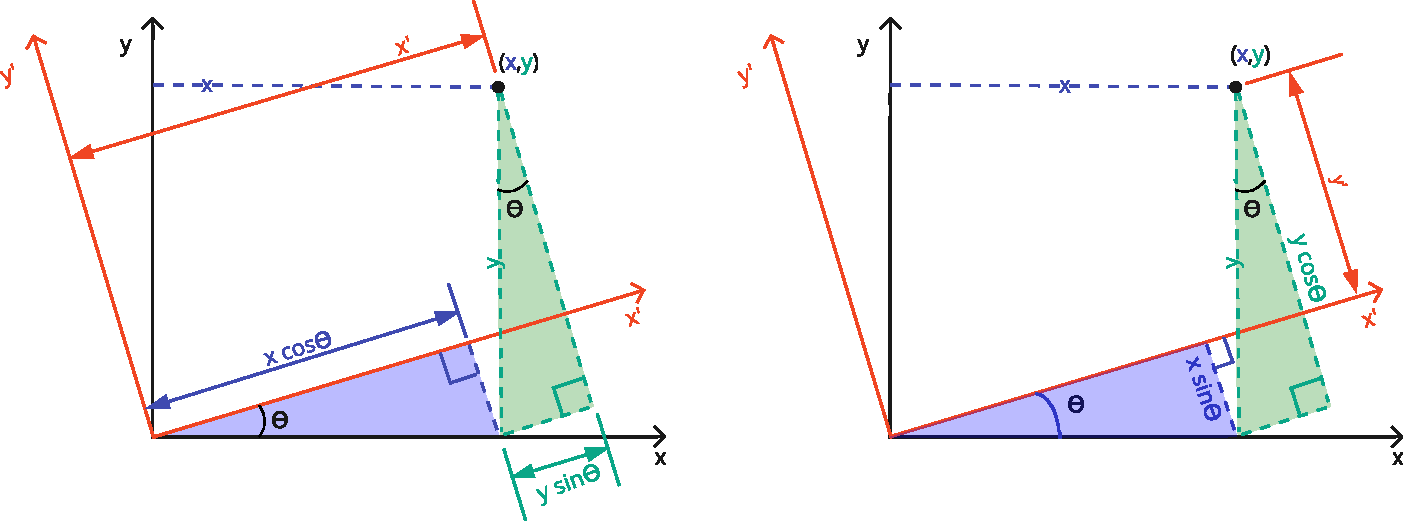
\includegraphics[width=1\linewidth]{so2}
    \caption{Rotación de coordenadas}
    \label{fig:rot}
\end{figure}

El módulo de este vector es invariante

\begin{align*}
    \boldsymbol{r}'\cdot\boldsymbol{r}' =&{x'}^2+{y'}^2  \\
    =&(x\cos\theta+y\sin\theta)^2+(y\cos\theta-x\sin\theta)^2\\
    = & x^2+y^2\,.
\end{align*}
Verifiquemos, bajo qué condiciones el módulo del vector de impulso es invariante bajo transformaciones de Lorentz. Definimos el producto escalar entre dos vectores
$\boldsymbol{b} = (b_1,b_2)$ y $\boldsymbol{c} = (c_1,c_2) $ como
\begin{align}
    \boldsymbol{b} \cdot \boldsymbol{c} = g_{1} b_1 c_1 + g_{2} b_2 c_2\,.
\end{align}
con $g_{1}$ y $g_{2}$ a ser fijados. 

Con esta definición el módulo del vector de impulso $\boldsymbol{b} = ({x^0},{x^1})$ en la base transformada, 
\begin{align*}
\boldsymbol{b}' = ({x^0}',{x^1}') = ({x^0}\cosh\xi - {x^1}\sinh\xi, {x^1}\cosh\xi -{x^0}\sinh\xi),
\end{align*}
es
\begin{align*}
    \boldsymbol{b}'\cdot\boldsymbol{b}' =& 
g_{1} {{x^0}'}^2 + g_{2} {{x^1}'}^2 \\
=& g_1\left({x^0}^2\cosh^2\xi -2 {x^0}{x^1}\cosh\xi\sinh\xi+{x^1}^2\sinh^2\xi\right)+
g_2\left({x^1}^2\cosh^2-2{x^0}{x^1}\cosh\xi\sinh\xi + {x^0}^2\sinh^2\xi\right).
\end{align*}
Si $g_1=1$ y $g_2=-1$, tenemos la definición del producto escalar en el espacio de Minkowski como
\begin{align}
\label{eq:mdp}
    \boldsymbol{b} \cdot \boldsymbol{c} \equiv b_1 c_1 - b_2 c_2\,,
\end{align}
y por lo tanto
\begin{align*}
    \boldsymbol{b}'\cdot\boldsymbol{b}' =& 
{{x^0}'}^2 - {{x^1}'}^2 \\
=& {x^0}^2(\cosh^2\xi-\sinh^2\xi)+{x^1}^2(\sinh^2-\cosh^2) -\cancel{2 {x^0}{x^1}\cosh\xi\sinh\xi}+\cancel{2 {x^0}{x^1}\cosh\xi\sinh\xi}\\
=&{x^0}^2 - {x^1}^2\,.
\end{align*}
Podemos ver que la invarianza del producto escalar bajo una transformación de Lorentz, fija la definición del producto escalar en ese espacio, como se da en la ec.~\eqref{eq:mdp}.

\begin{figure}
    \centering
    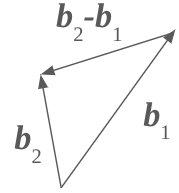
\includegraphics[scale=0.5]{b2-b1.png}
    \caption{$\Delta\boldsymbol{b} = \boldsymbol{b}_2 - \boldsymbol{b}_1$}
    \label{fig:b2-b1}
\end{figure}

Similarmente, para la diferencia de dos impulsos, como en la figura~\ref{fig:b2-b1}
\begin{align*}
    \Delta\boldsymbol{b} = \boldsymbol{b}_2 - \boldsymbol{b}_1 
\end{align*}
tiene un módulo que es invariante
\begin{align*}
    \Delta S^2 = |\Delta\boldsymbol{b}|^2=& |\boldsymbol{b}_2 -\boldsymbol{b}_1 |^2\\
    =&(\boldsymbol{b}_2 -\boldsymbol{b}_1)\cdot (\boldsymbol{b}_2 -\boldsymbol{b}_1)  \\
=&\left(t_2-t_1\right)^2 -\left(x_2-x_1\right)^2\\
    = &\Delta t^2 - \Delta x^2\,. 
\end{align*}
En el espacio completo tenemos
\begin{align*}
    \Delta S^2 =
     &c^2\Delta t^2 - \Delta x^2 - \Delta y^2 - \Delta z^2\,. 
\end{align*}

Definimos un vector en el espacio de Minkowski como
\begin{align*}
    x^\mu = (ct,x,y,z) = (ct,\boldsymbol{r})
\end{align*}

\section{Cuadrimomento}
En relatividad especial, la magnitud del vector momento para una partícula que se mueve a una velocidad $\boldsymbol{v}$, es
\begin{align*}
    p= \gamma m v\,.
\end{align*}
A continuación mostraremos porque se necesita el factor $\gamma$ en la ecuación para el momento. 

Si definimos el cuatrivector
\begin{align*}
    p^\mu = \left(\frac{E}{c},p_x,p_y,p_z\right) = \left(\frac{E}{c},\boldsymbol{p}\right),
\end{align*}
donde $c$ se comporta como un factor de conversión (al igual que $h$ cuando se necesite)
\begin{align*}
    \left[\frac{E}{c}\right] = \left[ M\frac{L^2}{T^2}\frac{T}{L}  \right] = \left[M \frac{L}{T}\right] = [p]\,,
\end{align*}
entonces esperamos que el módulo al cuadrado en el espacio de Minkowski, sea un invariante, una constante que llamaremos $m^2 c^4$ (en unidades de momento al cuadrado), tal que
\begin{align*}
    m^2 c^2 =& \frac{E^2}{c^2} - \boldsymbol{p}\cdot\boldsymbol{p} \\
        =&   \frac{E^2}{c^2} -p^2\,,
\end{align*}
donde $p^2 = |\boldsymbol{p}|^2 =\boldsymbol{p}\cdot\boldsymbol{p} $ en el espacio real en tres dimensiones.

Resolviendo para $E$
\begin{align*}
    \frac{E^2}{c^2} =& m^2c^2 + p^2\,.
\end{align*}
Resolviendo para $E^2$
\begin{align*}
        E^2 =& m^2 c^4 +  p^2c^2\\
         =& m^2 c^4 + \gamma^2 m^2 v^2 c^2\\
         =& m^2c^2(c^2+\gamma^2 v^2)\,.
\end{align*}
Usando la ecuación~\eqref{eq:gammasquare} para $\gamma^2$
\begin{align}
          E^2   =&m^2c^2\left[c^2+ \left(\frac{c^2}{c^2 - v^2}\right)v^2\right]\nonumber\\
         =& m^2 c^2\left(\frac{c^4-\cancel{c^2v^2}+\cancel{c^2v^2}}{c^2 - v^2}\right)\nonumber\\
         =& m^2c^2\frac{c^4}{c^2-v^2}\nonumber\\
         =& m^2c^4\frac{c^2}{c^2-v^2}\nonumber\\
         =& \gamma^2 m^2 c^4\,,
\end{align}

Por lo tanto
\begin{align}
    \boxed{E = \gamma m c^2\,.}
\end{align}
Usando la ecuación~\eqref{eq:gammasquare} para $\gamma$, tenemos
\begin{align}
    E = \frac{m c^2}{\sqrt{1-v^2/c^2}}
\end{align}

Hay dos límites:

\begin{enumerate}
    \item Límite no relativista: $m\gg p$ que resulta en 
    \begin{align*}
        E = m c^2\,,
    \end{align*}
    que la energía mínima que puede tener un objeto de masa $m$ y se denomina su \emph{energía en reposo}.
    \item Límite relativista: $m \ll p$ que resulta en
    \begin{align*}
        E = pc\,.
    \end{align*}

    Éste límite es válido para partículas con o sin masa (cómo el fotón).  En el caso de un fotón, hemos visto que su energía es 
    \begin{align}
        E=h\nu\,,
    \end{align}
    y reemplazando en la expresión anterior, tenemos que el momento de un fotón es 
    \begin{align}
        p=\frac{E}{c} =& \frac{h}{c}\nu\\
        [p] =& \left[\frac{E\cdot T}{\dfrac{L}{T}}\cdot \frac{1}{T}\right]\nonumber\\
         =& \left[\frac{M \dfrac{L^{\cancel{2}}}{T^{\cancel{2}}}\cdot \cancel{T}}{\cancel{\dfrac{L}{T}}}\cdot \frac{1}{\cancel{T}}\right]\nonumber\\
        = &\left[M \frac{L}{T}\right]\,,
    \end{align}
    como era de esperarse. 

    La longitud de onda de un fotón es
    \begin{align}
        \lambda =\frac{c}{\nu},,
    \end{align}
tal que $[\lambda] = [L]$ y por lo tanto
\begin{align}
    p =\frac{h}{\lambda}\,.
\end{align}
La correspondiente energía de un fotón de longitud de onda $\lambda$
\begin{align}
E = pc =\frac{hc}{\lambda}\,.    
\end{align}

    En el caso de una partícula relativista con masa, moviendose a una velocidad $v$, comparable a la velocidad de la luz
    \begin{align}
        E =&\gamma m v c \nonumber\\
        =& \frac{mvc}{\sqrt{1-v^2/c^2}}\,.
    \end{align}
    Por lo tanto
    \begin{align}
        \lim_{v\to c} E = \infty\,.
    \end{align}
\end{enumerate}
De modo que se requeriría  una energía infinita para acelerar un objeto material a la velocidad de la luz. 

Además, si aceptamos la existencia de una partícula que se pueda mover más rápido que la velocidad de la luz, llamada taquión, el radicando en el denominandor tendría un signo negativo y la energía sería imaginaria, lo que aparentemente no tiene significado físico. Es de anotar que a la fecha no se ha observado ningún taquión en la naturaleza.

\section{Ejemplos}
\begin{enumerate}
    \item Cálculo de Fotones por Segundo para Corte por Láser de CO\textsubscript{2}.

% --- Inicio del código LaTeX para insertar ---
Para un láser de CO\textsubscript{2} industrial de \SI{4000}{\watt} (\SI{4}{kW}), una potencia realista para cortar una placa de acero de \SI{20}{\milli\meter}, el número total de fotones que se acumulan en el punto de contacto es de aproximadamente:
\[ \boxed{N_{\text{fotones}} \approx \num{2.13e23} \text{ fotones por segundo}} \]
De estos, solo una pequeña fracción (alrededor del \SIrange{5}{10}{\percent}) es absorbida y utilizada para cortar el metal.

\subsection*{Desglose del Cálculo}
El proceso se divide en tres pasos principales:
\begin{enumerate}
    \item Calcular la energía de un único fotón de un láser de CO\textsubscript{2}.
    \item Estimar la energía necesaria por segundo para calentar, derretir y eliminar el acero.
    \item Combinar ambos resultados para encontrar el número de fotones por segundo.
\end{enumerate}

\subsubsection*{Paso 1: Energía de un Fotón de Láser de CO\textsubscript{2}}
La energía de un fotón ($E_{\text{fotón}}$) se calcula con la fórmula de Planck:
\[ E_{\text{fotón}} = \frac{hc}{\lambda} \]
Donde:
\begin{itemize}
    \item $h$ = Constante de Planck (\SI{6.626e-34}{\joule\second})
    \item $c$ = Velocidad de la luz (\SI{3e8}{\meter\per\second})
    \item $\lambda$ = Longitud de onda del láser de CO\textsubscript{2} (\SI{10.6}{\micro\meter} = \SI{10.6e-6}{\meter})
\end{itemize}
Sustituyendo los valores:
\[ E_{\text{fotón}} = \frac{(\SI{6.626e-34}{\joule\second}) \times (\SI{3e8}{\meter\per\second})}{\SI{10.6e-6}{\meter}} \approx \SI{1.875e-20}{\joule} \]

\subsubsection*{Paso 2: Estimación de la Energía Necesaria para Cortar el Acero}
La energía del láser debe calentar y derretir el acero. La potencia útil ($P_{\text{útil}}$) depende de la cantidad de material eliminado por segundo, lo cual depende de la velocidad de corte.

\paragraph{Suposición de Velocidad de Corte Realista:} Para acero de \SI{20}{\milli\meter}, una velocidad de corte típica es de \SI{0.8}{\meter\per\minute}.
\[ \text{Velocidad} = \SI{0.8}{\meter\per\minute} \div \SI{60}{\second\per\minute} \approx \SI{0.0133}{\meter\per\second} \]

\paragraph{Volumen de Acero Eliminado por Segundo ($V_{\text{seg}}$):}
El láser corta una ranura (kerf) con el diámetro del haz.
\begin{align*}
    V_{\text{seg}} &= (\text{espesor}) \times (\text{diámetro}) \times (\text{velocidad}) \\
    V_{\text{seg}} &= (\SI{20e-3}{\meter}) \times (\SI{0.1e-3}{\meter}) \times (\SI{0.0133}{\meter\per\second}) \approx \SI{2.66e-8}{\meter^3\per\second}
\end{align*}

\paragraph{Masa de Acero Eliminada por Segundo ($m_{\text{seg}}$):}
Usamos la densidad del acero ($\rho \approx \SI{7850}{\kilo\gram\per\meter^3}$).
\[ m_{\text{seg}} = V_{\text{seg}} \times \rho = (\SI{2.66e-8}{\meter^3\per\second}) \times (\SI{7850}{\kilo\gram\per\meter^3}) \approx \SI{2.08e-4}{\kilo\gram\per\second} \]

\paragraph{Cálculo de la Potencia Útil ($P_{\text{útil}}$):}
Necesitamos las propiedades térmicas del acero:
\begin{itemize}
    \item Calor específico ($c_p$): $\approx \SI{500}{\joule\per\kilo\gram\per\kelvin}$
    \item Punto de fusión: $\approx \SI{1500}{\celsius}$ (un $\Delta T$ de $\approx \SI{1480}{\celsius}$ desde $\SI{20}{\celsius}$)
    \item Calor latente de fusión ($L_f$): $\approx \SI{250000}{\joule\per\kilo\gram}$
\end{itemize}
\begin{align*}
    P_{\text{calentar}} &= m_{\text{seg}} \cdot c_p \cdot \Delta T = (\SI{2.08e-4}) \cdot 500 \cdot 1480 \approx \SI{154}{\watt} \\
    P_{\text{derretir}} &= m_{\text{seg}} \cdot L_f = (\SI{2.08e-4}) \cdot 250000 \approx \SI{52}{\watt}
\end{align*}
\[ P_{\text{útil}} = P_{\text{calentar}} + P_{\text{derretir}} \approx \SI{154}{\watt} + \SI{52}{\watt} = \SI{206}{\watt} \]
Esta es la potencia mínima teórica que el acero debe absorber.

\subsubsection*{Paso 3: Combinar Resultados y Asumir una Potencia de Láser}
La eficiencia de absorción de energía en el corte de acero grueso es baja (aprox. \SIrange{5}{10}{\percent}) debido a la reflexión y la conducción térmica.

Si asumimos una eficiencia del \SI{5.15}{\percent}, la potencia total requerida del láser ($P_{\text{total}}$) sería:
\[ P_{\text{total}} = \frac{P_{\text{útil}}}{\text{Eficiencia}} = \frac{\SI{206}{\watt}}{0.0515} \approx \SI{4000}{\watt} \]
Esto nos lleva a una suposición clave y realista: \textbf{se está utilizando un láser industrial de \SI{4}{kW}}.

\paragraph{Cálculo Final de Fotones por Segundo:}
El número de fotones por segundo ($N_{\text{fotones}}$) es la potencia total del láser dividida por la energía de cada fotón.
\[ N_{\text{fotones}} = \frac{P_{\text{total}}}{E_{\text{fotón}}} = \frac{\SI{4000}{\joule\per\second}}{\SI{1.875e-20}{\joule\per\text{fotón}}} \approx \num{2.13e23} \, \text{fotones/s} \]

\subsection*{Conclusión}
Aunque teóricamente solo se necesitan unos \SI{206}{\watt} de potencia absorbida para realizar el corte, debido a las ineficiencias del proceso, se requiere un láser mucho más potente. Para un láser industrial realista de \SI{4000}{\watt}, el haz deposita en el punto de contacto la asombrosa cantidad de \num{2.13e23} fotones cada segundo para lograr cortar la placa de acero de \SI{20}{\milli\meter}.

% --- Fin del código LaTeX ---
\item La Energía de la Fisión del Uranio

La primera bomba atómica, detonada en el proyecto Manhattan, funcionaba mediante la \textbf{fisión nuclear} del Uranio-235 (\textsuperscript{235}U). En este proceso, un neutrón lento golpea un núcleo de \textsuperscript{235}U, haciéndolo inestable. El núcleo se divide en dos núcleos más pequeños (llamados fragmentos de fisión), liberando varios neutrones y una enorme cantidad de energía.

El origen de esta energía es que la suma de las masas de los productos finales es \textbf{ligeramente menor} que la suma de las masas de los reactivos iniciales. Esta ``masa perdida'', conocida como \textbf{defecto de masa ($\Delta m$)}, se convierte íntegramente en energía según la famosa ecuación de Einstein.

\paragraph{Fórmula clave:}
\[ E = \Delta m c^2 \]

\subsection*{El Problema}
Considera una de las posibles reacciones de fisión del Uranio-235:
\[ \text{n} + {}^{235}\text{U} \rightarrow {}^{92}\text{Kr} + {}^{141}\text{Ba} + 3\text{n} + E \]

\paragraph{Datos (masas atómicas en reposo):}
\begin{itemize}
    \item Masa de un neutrón ($m_n$): \SI{1.00866}{\atomicmassunit}
    \item Masa de un átomo de Uranio-235 ($m_U$): \SI{235.04393}{\atomicmassunit}
    \item Masa de un átomo de Kriptón-92 ($m_{Kr}$): \SI{91.92615}{\atomicmassunit}
    \item Masa de un átomo de Bario-141 ($m_{Ba}$): \SI{140.91441}{\atomicmassunit}
\end{itemize}

\paragraph{Constantes:}
\begin{itemize}
    \item Unidad de masa atómica (u): $\SI{1}{\atomicmassunit} = \SI{1.6605e-27}{\kilo\gram}$
    \item Velocidad de la luz ($c$): $\SI{3e8}{\meter\per\second}$
\end{itemize}

\paragraph{Preguntas:}
\begin{enumerate}
    \item Calcula la energía liberada (en Joules) por la fisión de \textbf{un solo} átomo de Uranio-235.
    \item Estima la energía total liberada si \textbf{\SI{1}{\kilo\gram}} de Uranio-235 sufre una fisión completa.
\end{enumerate}

\subsection*{Solución Detallada}

\subsubsection*{Parte 1: Energía por un solo átomo de Uranio}

\paragraph{Paso 1: Calcular la masa total inicial ($m_{\text{inicial}}$)}
\[ m_{\text{inicial}} = m_n + m_U = \SI{1.00866}{\atomicmassunit} + \SI{235.04393}{\atomicmassunit} = \SI{236.05259}{\atomicmassunit} \]

\paragraph{Paso 2: Calcular la masa total final ($m_{\text{final}}$)}
\begin{align*}
    m_{\text{final}} &= m_{Kr} + m_{Ba} + 3 \times m_n \\
    &= \SI{91.92615}{\atomicmassunit} + \SI{140.91441}{\atomicmassunit} + 3 \times (\SI{1.00866}{\atomicmassunit}) \\
    &= \SI{91.92615}{\atomicmassunit} + \SI{140.91441}{\atomicmassunit} + \SI{3.02598}{\atomicmassunit} = \SI{235.86654}{\atomicmassunit}
\end{align*}

\paragraph{Paso 3: Calcular el Defecto de Masa ($\Delta m$)}
\[ \Delta m = m_{\text{inicial}} - m_{\text{final}} = \SI{236.05259}{\atomicmassunit} - \SI{235.86654}{\atomicmassunit} = \SI{0.18605}{\atomicmassunit} \]

\paragraph{Paso 4: Convertir el Defecto de Masa a Kilogramos}
\[ \Delta m_{\text{kg}} = \SI{0.18605}{\atomicmassunit} \times (\SI{1.6605e-27}{\kilo\gram\per\atomicmassunit}) \approx \SI{3.099e-28}{\kilo\gram} \]

\paragraph{Paso 5: Calcular la Energía Liberada ($E$)}
Aplicamos la fórmula $E = \Delta m c^2$:
\begin{align*}
    E &= (\SI{3.099e-28}{\kilo\gram}) \times (\SI{3e8}{\meter\per\second})^2 \\
    E &= (\SI{3.099e-28}) \times (\SI{9e16}) \, \si{\joule} \approx \SI{2.789e-11}{\joule}
\end{align*}
\textbf{Respuesta a la Pregunta 1:} La fisión de un solo átomo de U-235 libera aproximadamente \SI{2.79e-11}{\joule}.

\subsubsection*{Parte 2: Energía por \SI{1}{\kilo\gram} de Uranio}

\paragraph{Paso 6: Calcular el número de átomos en \SI{1}{\kilo\gram} de U-235}
\[ \text{Nº de átomos} \approx \frac{\SI{1}{\kilo\gram}}{\SI{235.04393}{\atomicmassunit} \times (\SI{1.6605e-27}{\kilo\gram\per\atomicmassunit})} \approx \num{2.56e24} \, \text{átomos} \]

\paragraph{Paso 7: Calcular la Energía Total Liberada}
\begin{align*}
    E_{\text{total}} &= (\SI{2.789e-11}{\joule\per\text{átomo}}) \times (\num{2.56e24} \, \text{átomos}) \\
    E_{\text{total}} &\approx \SI{7.14e13}{\joule}
\end{align*}
\textbf{Respuesta a la Pregunta 2:} La fisión completa de \SI{1}{\kilo\gram} de Uranio-235 liberaría aproximadamente \SI{71.4}{\tera\joule}.

\subsection*{Interpretación y Contexto: ¿Qué tan grande es esta energía?}
Para poner en perspectiva los \SI{71.4}{\tera\joule}:
\begin{itemize}
    \item \textbf{Equivalencia en TNT:} La energía liberada por la explosión de \SI{1}{\tonne} de TNT es de unos \SI{4.184}{\giga\joule} (\SI{4.184e9}{\joule}).
    \[ \text{Equivalente en TNT} = \frac{\SI{7.14e13}{\joule}}{\SI{4.184e9}{\joule\per\tonne}} \approx \num{17065} \text{ toneladas de TNT} \]
    Esto es comparable a la potencia de la bomba de Hiroshima (estimada entre 15 y 20 kilotones).
\end{itemize}

\paragraph{Conclusión del ejercicio:} Este problema demuestra claramente cómo la fórmula $E = \Delta m c^2$ se aplica en el mundo real. La aniquilación de una cantidad de masa casi imperceptible a nivel atómico (solo el \SI{0.08}{\percent} de la masa inicial se ``pierde''), al ser multiplicada por el gigantesco valor de $c^2$, se traduce en una liberación de energía de proporciones masivas.

% --- Fin del código LaTeX ---

% --- Inicio del código LaTeX para insertar ---

\item Energía de una Bomba de Fusión (Bomba de Hidrógeno)

Las armas termonucleares, o bombas de hidrógeno (H-bombs), liberan energía mediante la \textbf{fusión nuclear}, el mismo proceso que alimenta al Sol. En una bomba H, una bomba de fisión primaria genera las temperaturas y presiones extremas necesarias para forzar a los núcleos de isótopos ligeros de hidrógeno (como el Deuterio y el Tritio) a fusionarse.

La reacción de fusión más ``sencilla'' y una de las más energéticas es la fusión Deuterio-Tritio (D-T). Al igual que en la fisión, la energía proviene de un \textbf{defecto de masa}: la masa de los productos resultantes es ligeramente menor que la masa de los reactivos originales, y esta diferencia de masa se convierte en una cantidad colosal de energía.

\paragraph{Fórmula clave:}
\[ E = \Delta m c^2 \]

\subsection*{El Problema}
La reacción principal en muchas armas termonucleares es la fusión de un núcleo de Deuterio (${}^2\text{H}$) con uno de Tritio (${}^3\text{H}$):
\[ {}^2\text{H} + {}^3\text{H} \rightarrow {}^4\text{He} + \text{n} + E \]

\paragraph{Datos (masas nucleares en reposo):}
\begin{itemize}
    \item Masa de un núcleo de Deuterio (${}^2\text{H}$): \SI{2.014102}{\atomicmassunit}
    \item Masa de un núcleo de Tritio (${}^3\text{H}$): \SI{3.016049}{\atomicmassunit}
    \item Masa de un núcleo de Helio-4 (${}^4\text{He}$): \SI{4.002603}{\atomicmassunit}
    \item Masa de un neutrón (n): \SI{1.008665}{\atomicmassunit}
\end{itemize}

\paragraph{Constantes:}
\begin{itemize}
    \item Unidad de masa atómica (u): $\SI{1}{\atomicmassunit} = \SI{1.6605e-27}{\kilo\gram}$
    \item Velocidad de la luz ($c$): $\SI{3e8}{\meter\per\second}$
\end{itemize}

\paragraph{Preguntas:}
\begin{enumerate}
    \item Calcula la energía liberada (en Joules) por \textbf{una sola} reacción de fusión Deuterio-Tritio.
    \item Estima la energía total liberada si \textbf{\SI{1}{\kilo\gram}} de una mezcla equimolar (igual número de átomos de cada uno) de Deuterio y Tritio se fusiona completamente.
    \item Compara la energía liberada por kilogramo con la de la fisión del Uranio-235.
\end{enumerate}

\subsection*{Solución Detallada}

\subsubsection*{Parte 1: Energía por una sola reacción de fusión}

\paragraph{Paso 1: Calcular la masa total inicial ($m_{\text{inicial}}$)}
\[ m_{\text{inicial}} = m_{D} + m_{T} = \SI{2.014102}{\atomicmassunit} + \SI{3.016049}{\atomicmassunit} = \SI{5.030151}{\atomicmassunit} \]

\paragraph{Paso 2: Calcular la masa total final ($m_{\text{final}}$)}
\[ m_{\text{final}} = m_{He} + m_n = \SI{4.002603}{\atomicmassunit} + \SI{1.008665}{\atomicmassunit} = \SI{5.011268}{\atomicmassunit} \]

\paragraph{Paso 3: Calcular el Defecto de Masa ($\Delta m$)}
\[ \Delta m = m_{\text{inicial}} - m_{\text{final}} = \SI{5.030151}{\atomicmassunit} - \SI{5.011268}{\atomicmassunit} = \SI{0.018883}{\atomicmassunit} \]

\paragraph{Paso 4: Convertir el Defecto de Masa a Kilogramos}
\[ \Delta m_{\text{kg}} = \SI{0.018883}{\atomicmassunit} \times (\SI{1.6605e-27}{\kilo\gram\per\atomicmassunit}) \approx \SI{3.1455e-29}{\kilo\gram} \]

\paragraph{Paso 5: Calcular la Energía Liberada ($E$)}
\[ E = (\SI{3.1455e-29}{\kilo\gram}) \times (\SI{3e8}{\meter\per\second})^2 \approx \SI{2.831e-12}{\joule} \]
\textbf{Respuesta a la Pregunta 1:} Una sola reacción de fusión D-T libera aproximadamente \SI{2.83e-12}{\joule} (\SI{17.6}{\mega\electronvolt}).

\subsubsection*{Parte 2: Energía por \SI{1}{\kilo\gram} de combustible de fusión}

\paragraph{Paso 6: Calcular el número de reacciones en \SI{1}{\kilo\gram} de mezcla}
La masa de un ``par'' de combustible (D+T) es $m_{\text{par}} = \SI{5.030151}{\atomicmassunit} \approx \SI{8.3526e-27}{\kilo\gram}$.
\[ \text{Nº de reacciones} = \frac{\SI{1}{\kilo\gram}}{\SI{8.3526e-27}{\kilo\gram}} \approx \num{1.197e26} \, \text{reacciones} \]

\paragraph{Paso 7: Calcular la Energía Total Liberada}
\[ E_{\text{total}} = (\SI{2.831e-12}{\joule\per\text{reacción}}) \times (\num{1.197e26} \, \text{reacciones}) \approx \SI{3.388e14}{\joule} \]
\textbf{Respuesta a la Pregunta 2:} La fusión completa de \SI{1}{\kilo\gram} de mezcla D-T liberaría aproximadamente \SI{339}{\tera\joule}.

\subsubsection*{Parte 3: Comparación con la Fisión}

\paragraph{Paso 8: Comparar la Energía por Kilogramo}
\begin{itemize}
    \item \textbf{Energía de Fusión (por kg):} \SI{3.39e14}{\joule}
    \item \textbf{Energía de Fusión (por kg, de ejercicio anterior):} \SI{7.14e13}{\joule}
\end{itemize}
\[ \frac{\text{Energía Fusión}}{\text{Energía Fisión}} = \frac{\SI{3.39e14}{\joule}}{\SI{7.14e13}{\joule}} \approx 4.75 \]
\textbf{Respuesta a la Pregunta 3:} La fusión de \SI{1}{\kilo\gram} de combustible D-T libera aproximadamente \textbf{4.75 veces más energía} que la fisión de \SI{1}{\kilo\gram} de Uranio-235.

\subsection*{Eficiencia de una Bomba de Hidrógeno}

La eficiencia de una bomba de hidrógeno para ``quemar'' o fusionar todo su combustible de fusión es sorprendentemente baja. Generalmente, la eficiencia de la etapa de fusión en un arma termonuclear moderna se encuentra en el rango del \SIrange{20}{40}{\percent}. Esto significa que entre el \SIrange{60}{80}{\percent} del combustible de fusión es simplemente dispersado por la explosión sin reaccionar.

\subsubsection*{¿Por qué la Eficiencia no es del 100\%? El Principio de "Desmontaje Explosivo"}

El factor limitante más importante en cualquier arma nuclear es que \textbf{la propia explosión destruye las condiciones necesarias para que la reacción continúe}.
\begin{enumerate}
    \item \textbf{Condiciones Extremas:} Para que la fusión ocurra, el combustible debe ser comprimido a densidades enormes y calentado a temperaturas de decenas de millones de grados Celsius, lo cual se logra con una explosión de fisión primaria.
    \item \textbf{La Carrera Contra el Tiempo:} En el instante en que la fusión comienza, libera una energía aún más colosal. Esta energía crea una presión y una onda de choque expansiva que viaja hacia afuera.
    \item \textbf{El Desmontaje:} Esta fuerza expansiva trabaja directamente en contra de la fuerza de implosión que mantiene el combustible comprimido. Tan pronto como la presión hacia afuera supera la presión de confinamiento, el combustible se expande rápidamente.
    \item \textbf{"Apagado" de la Reacción:} A medida que el combustible se expande, su densidad y temperatura caen en picado. En cuestión de nanosegundos, las condiciones caen por debajo del umbral necesario para la fusión, y la reacción se detiene.
\end{enumerate}
La eficiencia es, por lo tanto, una medida de cuán bien el diseño puede \textbf{mantener el combustible confinado} antes de que la inevitable explosión lo desmonte todo.

\subsubsection*{Ejemplo Numérico Ilustrativo}
Imaginemos una bomba de \SI{1}{\mega\tonne} de TNT ($\approx \SI{4.184e15}{\joule}$), donde el \SI{50}{\percent} de la energía proviene de la fusión (\SI{500}{\kilo\tonne} o $\approx \SI{2.092e15}{\joule}$).

\paragraph{1. Masa de combustible que SÍ se fusionó:}
\[ \text{Masa fusionada} = \frac{\text{Energía liberada}}{\text{Energía por kg}} = \frac{\SI{2.092e15}{\joule}}{\SI{3.39e14}{\joule\per\kilo\gram}} \approx \SI{6.17}{\kilo\gram} \]

\paragraph{2. Masa total de combustible en la bomba:}
Si asumimos una eficiencia de fusión plausible del \SI{30}{\percent}:
\[ \text{Masa total} = \frac{\text{Masa fusionada}}{\text{Eficiencia}} = \frac{\SI{6.17}{\kilo\gram}}{0.30} \approx \SI{20.6}{\kilo\gram} \]
Esto significa que para que \SI{6.17}{\kilo\gram} de combustible reaccionen, la bomba debe estar cargada con más de \SI{20}{\kilo\gram}. El resto se dispersa sin reaccionar.

\subsubsection*{Comparación con las Bombas de Fisión}
La eficiencia de las bombas de fisión puras es generalmente aún menor:
\begin{itemize}
    \item \textbf{Bomba de tipo "cañón" (Hiroshima):} Extremadamente ineficiente, con solo un \SI{1.7}{\percent} de eficiencia de fisión.
    \item \textbf{Bomba de tipo "implosión" (Nagasaki):} Mucho más eficiente, pero aún baja, con una eficiencia estimada del \SIrange{15}{20}{\percent}.
\end{itemize}
La eficiencia de la fusión en una bomba H, aunque baja, es considerablemente mayor gracias al ingenioso método de implosión por radiación, que confina el combustible de manera mucho más intensa.

% --- Fin del código LaTeX ---

\item Calcule el producto escalar de Lorentz para el cuadrivector de momento
\begin{align*}
    p^\mu = \left(\frac{E}{c},p_x,p_y,p_z\right),
\end{align*}
donde la energía y la magnitud del vector $\boldsymbol{p} = (p_x,p_y,p_z)$ son
\begin{align*}
    E =&\gamma m c^2\,, & p=&\gamma m v \,.
\end{align*}


\end{enumerate}

\section{Leyes de Newton}
\begin{enumerate}
    \item Si un objeto cambia su  cantidad de movimiento durante un intervalo de tiempo $\Delta t$, es porque existe una fuerza neta actuando sobre él durante ese intervalo.  Dicha fuerza viene dada por
    \begin{align}
        \boldsymbol{F} = \frac{\Delta \boldsymbol{p}}{\Delta t}
    \end{align}
    donde
    \begin{align}
    \Delta t =& t_{\text{final}}-t_{\text{inicial}}\\
    \Delta\boldsymbol{p} =& \boldsymbol{p}_{\text{final}}
    - \boldsymbol{p}_{\text{inicial}}\,.    
    \end{align}

\item  para cada fuerza (acción) que un objeto ejerce sobre otro, existe una fuerza de igual magnitud y dirección opuesta (reacción)
\end{enumerate}

Durante ese intervalo de tiempo el objeto se desplazo una distancia
\begin{align}
    \Delta\boldsymbol{r} =& \boldsymbol{r}_{\text{final}}
    - \boldsymbol{r}_{\text{inicial}}\,.      
\end{align}
%analisis dimensional
Podemos entonces definir una cantidad escalar que tiene unidades de energía que llamaremos trabajo
\begin{align}
    W = \boldsymbol{F}\cdot \Delta\boldsymbol{r}\,.
\end{align}




Para una partícula de masa $m$ que se mueve a velocidad $\boldsymbol{v}$, su inercia, o cantidad de movimiento, o momento, es
\begin{align}
    \boldsymbol{p} = \gamma m \boldsymbol{v}\,.
\end{align}





\section{Límite no relativista}

Para el momento es suficiente hacer $\gamma \approx 1$
\begin{align}
    \boldsymbol{p} \approx m \boldsymbol{v}\,.
\end{align}


Para la energía, podemos usar
\begin{align*}
    (1+x)^n \approx 1+nx\,,\qquad\text{si $x\ll 1$}\,,
\end{align*}
tenemos que en el límite no relativista correspondiente a 
\begin{align*}
    \frac{v^2}{c^2} \ll 1\,,
\end{align*}
podemos aproximar el factor de Lorentz $\gamma$ de la siguiente manera
\begin{align}
    \gamma =&\frac{1}{\sqrt{1-v^2/c^2}}\nonumber\\
    =& \left(1-\frac{v^2}{c^2}\right)^{-1/2}\nonumber\\
    \approx& 1+\frac{v^2}{2c^2}\,.
\end{align}


En la ecuación para la energía de una partícula de masa $m$ moviéndose a una velocidad $v$, tenemos que
\begin{align*}
    E =& \gamma m c^2\nonumber\\
     \approx& \left(1+\frac{v^2}{c^2}\right)mc^2\nonumber\\
      E=&mc^2 + \frac{1}{2}m v^2\,,
\end{align*}
donde 
\begin{align}
    \text{Energía en reposo:}\qquad& E_0 = mc^2\,,\\
     \text{Energía cinética:}\qquad& K = \frac{1}{2}mv^2\,.
\end{align}

Note que el concepto de energía cinética aplica sólo en el caso no relativista.

Note que la diferencia de energía es
\begin{align}
    \Delta E =& E_{\text{final}} -E_{\text{inicial}} \nonumber\\
    =& \cancel{mc^2} + \frac{1}{2}mv^2_{\text{final}} -\cancel{mc^2} - \frac{1}{2}mv^2_{\text{inicial}}\nonumber\\
=& \frac{1}{2}mv^2_{\text{final}} - \frac{1}{2}mv^2_{\text{inicial}}\nonumber\\
=& K_\text{final} -K_\text{inicial} \nonumber\\
=& \Delta K\,.
\end{align}

Teorema de trabajo y energía
\begin{align}
    W =& \Delta K\nonumber\\
    =& \frac{1}{2}mv^2_{\text{final}} - \frac{1}{2}mv^2_{\text{inicial}}\,.
\end{align}
Lo que realmente tiene sentido físico es la diferencia de energías.

\subsection{Aceleración constante}


En una dimensión, $x$, con $F$ constante, $t_{\text{inicial}} = 0$ y $t_{\text{final}} = 0$, $v_{\text{inicial}} = v_0$ y $v_{\text{final}} = v$

\begin{align}
    v_0 = \pm a t =\pm \frac{F}{m} t
\end{align}

\begin{align}
    v = v_0 \pm\frac{F}{m} t
\end{align}

\begin{align*}
    \pm F\Delta x =& \frac{1}{2}mv^2 - \frac{1}{2}mv^2_0\\
    =&\frac{1}{2}m \left(v_0 \pm\frac{F}{m} t\right)^2 - 
    \frac{1}{2}mv^2_0\\
    =& \pm v_0 t F +\frac{1}{2}\frac{F^2}{m} t^2
\end{align*}

\begin{align*}
    \Delta x = x-x_0 = v_0 t \pm \frac{1}{2}\frac{F}{m} t^2\,.
\end{align*}

\begin{align}
    x = x_0 + v_0 t \pm \frac{1}{2}\frac{F}{m} t^2
\end{align}
\appendix

\section*{Apendices}


\section{Movimiento Relativista y No Relativista Bajo una Fuerza Constante}
Esta sección proporciona un análisis completo del movimiento de una partícula con velocidad inicial en dos dimensiones bajo la influencia de una fuerza constante en una dirección. Primero derivamos la ecuación de movimiento completamente relativista, luego la expresamos elegantemente en términos de la energía total relativista, revelando su conexión con el Teorema del Trabajo y la Energía. Posteriormente, demostramos el principio de correspondencia mostrando cómo la ecuación relativista se reduce correctamente al caso clásico en el límite no relativista. Finalmente, para completar, derivamos la ecuación de movimiento clásica de forma independiente utilizando el Teorema del Trabajo y la Energía no relativista.

\subsection{Configuración del Problema}
Consideramos el movimiento de una partícula de masa en reposo $m$.
\begin{itemize}
    \item \textbf{Condiciones Iniciales:} En el tiempo $t=0$, la partícula está en la posición $(x_0, y_0)$ con una velocidad inicial $\boldsymbol{u}_0 = (u_{x0}, u_{y0})$.
    \item \textbf{Fuerza:} Una fuerza constante $\boldsymbol{F}$ actúa solo en la dirección y negativa: $\boldsymbol{F} = (0, -F)$, donde $F$ es una constante positiva.
\end{itemize}
En relatividad, la Segunda Ley de Newton se escribe como la tasa de cambio del momento relativista:
\[ \boldsymbol{F} = \frac{d\boldsymbol{p}}{dt}, \quad \text{donde} \quad \boldsymbol{p} = \gamma m \boldsymbol{u} \]
El factor de Lorentz, $\gamma$, depende de la velocidad total $u = \sqrt{u_x^2 + u_y^2}$:
\[ \gamma = \frac{1}{\sqrt{1 - u^2/c^2}} = \frac{1}{\sqrt{1 - (u_x^2 + u_y^2)/c^2}} \]
Esta dependencia de la velocidad total significa que el movimiento en las direcciones x e y está acoplado, una característica clave de la dinámica relativista.

\subsection{La Ecuación de Movimiento Relativista}

\subsection{Resolviendo para el Momento}
La ecuación vectorial $\boldsymbol{F} = d\boldsymbol{p}/dt$ proporciona dos ecuaciones escalares para las componentes del momento $p_x$ y $p_y$.
\begin{itemize}
    \item \textbf{Dirección x:} $F_x = \frac{dp_x}{dt} = 0$. Esto implica que la componente x del momento se conserva:
    \[ p_x(t) = p_{x0} = \gamma_0 m u_{x0} \]
    donde $\gamma_0$ es el factor de Lorentz inicial.
    \item \textbf{Dirección y:} $F_y = \frac{dp_y}{dt} = -F$. Integrando con respecto al tiempo se obtiene:
    \[ p_y(t) = p_{y0} - Ft = \gamma_0 m u_{y0} - Ft \]
\end{itemize}

\subsection{Encontrando la Velocidad \texorpdfstring{$u_y(t)$}{uy(t)}}
Para encontrar la ecuación de movimiento para $y(t)$, primero necesitamos la velocidad $u_y(t) = dy/dt$. Podemos expresar las componentes de la velocidad en términos del momento y la energía total usando la relación relativista energía-momento $E^2 = (pc)^2 + (mc^2)^2$. Dado que $E=\gamma m c^2$, podemos encontrar $\gamma = \frac{1}{mc}\sqrt{p_x^2 + p_y^2 + m^2c^2}$. Esto conduce a:
\[ u_y(t) = \frac{p_y(t)}{\gamma(t) m} = \frac{c \, p_y(t)}{\sqrt{p_x(t)^2 + p_y(t)^2 + m^2c^2}} \]
Sustituyendo nuestras expresiones dependientes del tiempo para el momento:
\[ \frac{dy}{dt} = u_y(t) = \frac{c (p_{y0} - Ft)}{\sqrt{p_{x0}^2 + (p_{y0} - Ft)^2 + m^2c^2}} \]

\subsection{Integrando para Encontrar la Posición \texorpdfstring{$y(t)$}{y(t)}}
Integramos la velocidad $u_y(t)$ de $0$ a $t$ para encontrar el desplazamiento.
\[ y(t) - y_0 = \int_0^t \frac{c (p_{y0} - Ft')}{\sqrt{p_{x0}^2 + (p_{y0} - Ft')^2 + m^2c^2}} \, dt' \]
Esta integral se puede resolver usando una sustitución u para el término dentro de la raíz cuadrada. El resultado de la integración es:
\[ y(t) - y_0 = \frac{c}{F} \left( \sqrt{p_{x0}^2 + p_{y0}^2 + m^2c^2} - \sqrt{p_{x0}^2 + (p_{y0} - Ft)^2 + m^2c^2} \right) \]
Esto da la ecuación de movimiento relativista final para la coordenada y.

\subsection{Teorema del Trabajo y la Energía}

\begin{equation}
dW = \overline{F} \cdot d\overline{s} \label{eq:3}
\end{equation}
es el trabajo infinitesimal realizado por la fuerza $\overline{F}$ mientras la partícula sufre el desplazamiento $d\overline{s}$ a lo largo de su trayectoria. Usamos la segunda ley de Newton del movimiento
\begin{equation}
\overline{F} = \frac{d(m\overline{v})}{dt}
\end{equation}
en la ecuación (\ref{eq:3}) para obtener una expresión para el trabajo infinitesimal
\begin{align*}
dW &= \frac{d(m\overline{v})}{dt} \cdot \overline{v}dt \\
&= \frac{d}{dt}\left(\frac{1}{2}m\overline{v}\cdot\overline{v}\right)dt \\
&= d\left(\frac{1}{2}m\overline{v}^{2}\right).
\end{align*}
Dado que la cantidad escalar $\frac{1}{2}m\overline{v}^{2}$ es la energía cinética de la partícula, se sigue que
\begin{equation}
dW = dT. \label{eq:4}
\end{equation}
La ecuación (\ref{eq:4}) es la forma diferencial del teorema del trabajo y la energía: establece que el trabajo diferencial de la resultante de las fuerzas que actúan sobre una partícula es igual, en cualquier momento, al cambio diferencial en la energía cinética de la partícula. Integrando la ecuación (\ref{eq:4}) entre el punto 1 y el punto 2, correspondientes a las velocidades $\overline{v}_1$ y $\overline{v}_2$ de la partícula, obtenemos
\begin{equation}
W_{12} = \int_{1}^{2} dW = \int_{1}^{2} dT = T_2 - T_1 = \frac{1}{2}m\overline{v}_{2}^{2} - \frac{1}{2}m\overline{v}_{1}^{2}. \label{eq:5}
\end{equation}



\subsection{Formulación Energética de la Ecuación Relativista}
La ecuación anterior se puede expresar de una forma mucho más elegante y físicamente perspicaz utilizando el concepto de energía total relativista.
Sea $E_0$ la energía total inicial en $t=0$:
\[ E_0 = \sqrt{(p_{x0}^2 + p_{y0}^2)c^2 + (mc^2)^2} \]
Y sea $E(t)$ la energía total en el tiempo $t$:
\[ E(t) = \sqrt{(p_x(t)^2 + p_y(t)^2)c^2 + (mc^2)^2} = \sqrt{(p_{x0}^2 + (p_{y0}-Ft)^2)c^2 + (mc^2)^2} \]
Podemos ver que los términos en nuestra ecuación para $y(t)$ son simplemente $E_0/c$ y $E(t)/c$. Sustituyendo esto se obtiene:
\[ y(t) - y_0 = \frac{c}{F} \left( \frac{E_0}{c} - \frac{E(t)}{c} \right) \]
El factor $c$ se cancela, lo que lleva a la forma notablemente simple:
\[ \boxed{y(t) = y_0 + \frac{E_0 - E(t)}{F}} \]
Esta ecuación es una declaración directa del Teorema del Trabajo y la Energía, $F \Delta y = -\Delta E$, con la energía relativista en lugar de la energía cinética, ver más abajo.

\subsection{El Límite No Relativista (Principio de Correspondencia)}
Una teoría relativista válida debe reproducir los resultados clásicos a bajas velocidades ($u \ll c$). Mostramos esto usando la aproximación binomial para la energía total $E = \gamma mc^2$. Para velocidades pequeñas, $\gamma \approx 1 + \frac{1}{2}\frac{u^2}{c^2}$, lo que da:
\[ E \approx mc^2 + \frac{1}{2}mu^2 = (\text{Energía en Reposo}) + (\text{Energía Cinética Clásica}) \]
Aplicando esto a nuestra ecuación de movimiento basada en la energía:
\[ y(t) - y_0 = \frac{1}{F} \left[ \left(mc^2 + \frac{1}{2}mu_0^2\right) - \left(mc^2 + \frac{1}{2}mu(t)^2\right) \right] = \frac{m}{2F}(u_0^2 - u(t)^2) \]
En el límite no relativista, las velocidades son $u_x(t) = u_{x0}$ y $u_y(t) = u_{y0} - \frac{F}{m}t$. Sustituyendo esto:
\begin{align*}
y(t) - y_0 &= \frac{m}{2F} \left[ (u_{x0}^2 + u_{y0}^2) - \left(u_{x0}^2 + (u_{y0} - \frac{F}{m}t)^2\right) \right] \\
&= \frac{m}{2F} \left[ u_{y0}^2 - \left(u_{y0}^2 - 2u_{y0}\frac{F}{m}t + \frac{F^2}{m^2}t^2\right) \right] \\
&= \frac{m}{2F} \left[ 2u_{y0}\frac{F}{m}t - \frac{F^2}{m^2}t^2 \right] \\
&= u_{y0}t - \frac{F}{2m}t^2
\end{align*}
Esto produce la ecuación de movimiento clásica final:
\[ \boxed{y(t) = y_0 + u_{y0}t - \frac{F}{2m}t^2} \]
La fórmula relativista se reduce correctamente a la clásica.

\subsection{Derivación Directa del Caso No Relativista}
Como confirmación final, podemos derivar la ecuación de movimiento clásica directamente del Teorema del Trabajo y la Energía no relativista, $W_{neto} = \Delta K$.
\begin{itemize}
    \item \textbf{Trabajo Realizado:} $W_{neto} = \boldsymbol{F} \cdot \Delta\boldsymbol{r} = -F(y(t) - y_0)$.
    \item \textbf{Cambio en la Energía Cinética:} $\Delta K = K_{final} - K_{inicial} = \frac{1}{2}mu(t)^2 - \frac{1}{2}mu_0^2$.
\end{itemize}
Usando las velocidades clásicas $u_x(t) = u_{x0}$ y $u_y(t) = u_{y0} - \frac{F}{m}t$:
\[ \Delta K = \frac{1}{2}m\left[ (u_{x0}^2 + (u_{y0}-\frac{F}{m}t)^2) - (u_{x0}^2+u_{y0}^2) \right] = \frac{1}{2}m\left[ (u_{y0}-\frac{F}{m}t)^2 - u_{y0}^2 \right] \]
Estableciendo $W_{neto} = \Delta K$:
\[ -F(y(t)-y_0) = \frac{1}{2}m\left[ (u_{y0}^2 - 2u_{y0}\frac{F}{m}t + \frac{F^2}{m^2}t^2) - u_{y0}^2 \right] \]
\[ -F(y(t)-y_0) = -u_{y0}Ft + \frac{F^2}{2m}t^2 \]
Dividiendo por $-F$ se obtiene el resultado idéntico:
\[ y(t) - y_0 = u_{y0}t - \frac{F}{2m}t^2 \]







% --- INFORMACIÓN DEL TÍTULO ---
\section{Derivación de las Transformaciones de Lorentz a partir de Simetrías del Espacio--tiempo}
\label{sec:tl}
\subsection{El Enfoque de Ignatowski}
Este documento presenta una derivación de las transformaciones de Lorentz basada en principios fundamentales de simetría, en lugar de postular la constancia de la velocidad de la luz. Este enfoque, a veces llamado la derivación de Ignatowski, se basa en el Principio de Relatividad y la homogeneidad e isotropía del espaciotiempo. Mostraremos que estos principios conducen lógicamente a la existencia de una velocidad universal e invariante, que identificamos con la velocidad de la luz.

Ver \cite{Datta:2022cpw} %https://inspirehep.net/literature/2611550


\subsection{Principios Fundamentales}
La derivación se basa en tres supuestos centrales:
\begin{enumerate}
    \item \textbf{El Principio de Relatividad:} Las leyes de la física son las mismas en todos los sistemas de referencia inerciales.
    \item \textbf{Homogeneidad del Espaciotiempo:} Las leyes de la física son independientes de la posición en el espacio y el tiempo.
    \item \textbf{Isotropía del Espacio:} Las leyes de la física son independientes de la dirección.
\end{enumerate}


\subsection{Paso 1: Linealidad a partir de la Homogeneidad}
Consideremos dos sistemas de referencia inerciales, $S(x,t)$ y $S'(x',t')$, con $S'$ moviéndose a una velocidad $v$ relativa a $S$ a lo largo del eje x. Buscamos las funciones de transformación $x' = f(x,t)$ y $t' = g(x,t)$.

La homogeneidad del espaciotiempo implica que las ecuaciones de transformación deben ser \textbf{lineales}. Si no lo fueran, un movimiento uniforme en un sistema (una línea recta en un diagrama de espaciotiempo) aparecería como un movimiento acelerado en otro. Esto significaría que las leyes de la física dependerían de la elección del origen, violando la homogeneidad. Por lo tanto, la forma más general de las transformaciones debe ser lineal:
\begin{align*}
x' &= Ax + Bt \\
t' &= Dx + Et
\end{align*}
donde los coeficientes $A, B, D, E$ solo pueden depender de la velocidad relativa, $v$.

\subsection{Paso 2: Usando Cinemática Básica}
Podemos simplificar los coeficientes usando el movimiento de los orígenes de los sistemas.
\begin{itemize}
    \item El origen del sistema $S'$ ($x'=0$) se mueve con velocidad $v$ en el sistema $S$. Su posición en $S$ es por lo tanto $x=vt$. Sustituyamos esto en nuestra primera ecuación:
    \[ 0 = A(vt) + Bt \implies 0 = (Av+B)t \]
    Esto debe ser válido para todo tiempo $t$, por lo que debemos tener $B = -Av$. La transformación para $x'$ se convierte en:
    \[ x' = Ax - Avt = A(x-vt) \]
\end{itemize}
Renombremos el coeficiente $A(v)$ con la notación más familiar $\gamma(v)$.
\begin{equation} \label{eq:x_prime}
x' = \gamma(v)(x - vt)
\end{equation}

\subsection{Paso 3: Aplicando la Relatividad y la Isotropía}
El Principio de Relatividad establece que la transformación de $S'$ de vuelta a $S$ debe tener exactamente la misma forma matemática. La única diferencia es que desde la perspectiva de $S'$, el sistema $S$ se mueve con velocidad $-v$. Por lo tanto, la transformación inversa debe ser:
\begin{equation} \label{eq:x}
x = \gamma(-v)(x' + vt')
\end{equation}
Ahora, invocamos la \textbf{isotropía del espacio}. La isotropía significa que la física no debe depender de la dirección del vector velocidad. Por lo tanto, cualquier efecto físico de la transformación solo puede depender de la \textit{rapidez}, $|v|$, no de la dirección de la velocidad. Esto implica:
\[ \gamma(v) = \gamma(-v) \]
Esto simplifica nuestro par de transformaciones a:
\begin{align*}
x' &= \gamma(v)(x - vt) \\
x &= \gamma(v)(x' + vt')
\end{align*}

\subsection{Paso 4: Encontrando la Transformación del Tiempo}
Todavía necesitamos determinar la transformación para el tiempo. Podemos mostrar que debe tomar la forma simétrica:
\begin{equation} \label{eq:t_prime}
t' = \gamma(v)(t - \alpha(v) x)
\end{equation}
donde $\alpha(v)$ es alguna función de la velocidad. Por el Principio de Relatividad, la transformación inversa debe ser:
\begin{equation} \label{eq:t}
t = \gamma(v)(t' + \alpha(v) x')
\end{equation}
Nótese que la isotropía implica $\alpha(-v) = -\alpha(v)$ (debe ser una función impar).

\subsection{Paso 5: La Propiedad de Grupo y la Constante Universal}
Este es el paso crucial que reemplaza el postulado de la velocidad de la luz. Consideremos tres sistemas: $S$, $S'$ y $S''$. Sea la velocidad de $S'$ relativa a $S$ $v_1$, y la velocidad de $S''$ relativa a $S'$ $v_2$. La composición de estas dos transformaciones debe dar como resultado una transformación de la misma forma.

Sustituyendo (\ref{eq:x_prime}) y (\ref{eq:t_prime}) en (\ref{eq:x}) y (\ref{eq:t}), podemos resolver para las funciones. Un método más directo es requerir consistencia entre las transformaciones. Sustituyamos (\ref{eq:x_prime}) en (\ref{eq:x}):
\begin{align*}
x &= \gamma(v)(x' + vt') \\
x &= \gamma(v)[\gamma(v)(x-vt) + v t']
\end{align*}
Ahora sustituimos nuestra expresión para $t'$ (\ref{eq:t_prime}):
\begin{align*}
x &= \gamma(v)[\gamma(v)(x-vt) + v \gamma(v)(t - \alpha(v)x)] \\
x &= \gamma(v)^2 [ (x-vt) + v(t-\alpha(v)x) ] \\
x &= \gamma(v)^2 [ x - vt + vt - v\alpha(v)x ] \\
x &= \gamma(v)^2 x (1 - v\alpha(v))
\end{align*}
Como esto debe ser válido para cualquier $x$, debemos tener:
\[ 1 = \gamma(v)^2 (1 - v\alpha(v)) \]
Esto relaciona nuestras dos funciones desconocidas, $\gamma(v)$ y $\alpha(v)$.

A partir del argumento de la propiedad de grupo (considerando tres sistemas), se puede mostrar que la razón $\alpha(v)/v$ debe ser una constante universal, independiente del sistema de referencia. Llamemos a esta constante $K$.
\[ \frac{\alpha(v)}{v} = K \implies \alpha(v) = Kv \]
Ahora sustituimos esto de nuevo en nuestra relación de consistencia:
\[ 1 = \gamma(v)^2 (1 - v(Kv)) = \gamma(v)^2 (1 - K v^2) \]
Resolviendo para $\gamma(v)$:
\[ \boxed{\gamma(v) = \frac{1}{\sqrt{1 - K v^2}}} \]

\subsection{Paso 6: La Naturaleza Física de la Constante \texorpdfstring{$K$}{K}}
Hemos derivado la forma completa de las transformaciones basándonos únicamente en principios de simetría. La física está contenida en la constante universal $K$.
\begin{enumerate}
    \item \textbf{Caso 1: $K=0$} \\
    Si $K=0$, entonces $\gamma = 1$ y $\alpha=0$. Las transformaciones se convierten en $x' = x - vt$ y $t'=t$. Esta es la \textbf{transformación de Galileo}. En este universo, no hay límite de velocidad.

    \item \textbf{Caso 2: $K<0$} \\
    Si $K$ es negativo, sea $K = -1/R^2$. Entonces $\gamma = 1/\sqrt{1+v^2/R^2}$. Esto corresponde a transformaciones en un espacio euclidiano 4D (rotaciones). Esto es matemáticamente posible pero no describe nuestro universo.

    \item \textbf{Caso 3: $K>0$} \\
    Si $K$ es positivo, debe tener unidades de (1/velocidad$^2$). Definamos una nueva constante $c$ tal que $K = 1/c^2$. Esta constante $c$ debe ser una velocidad universal e invariante. El factor de Lorentz y las transformaciones se convierten en:
    \[ \gamma = \frac{1}{\sqrt{1 - v^2/c^2}} \]
    \[ x' = \gamma(x-vt) \]
    \[ t' = \gamma(t - \frac{v}{c^2}x) \]
    Estas son las \textbf{transformaciones de Lorentz}.
\end{enumerate}

\subsection{Conclusión}
Sin asumir nunca que la luz viaja a una velocidad constante, hemos demostrado que las simetrías fundamentales del espaciotiempo (homogeneidad e isotropía) y el principio de relatividad conducen a una conclusión sorprendente: \textbf{debe existir una velocidad universal e invariante en nuestro universo}.

Toda la evidencia experimental, desde el electromagnetismo hasta la desintegración de partículas, confirma que vivimos en un universo donde $K > 0$. Llamamos a esta velocidad universal $c$, y la identificamos con la velocidad de la luz en el vacío. La constancia de la velocidad de la luz no es una suposición separada, sino una consecuencia directa de la estructura del espaciotiempo mismo.


\section{Número Imaginario}
Definimos
\begin{align}
    i \equiv \sqrt{-1}\,.
\end{align}
Por lo tanto
\begin{align}
    i^2 = i\cdot i = (-1)^{\frac{1}{2}}(-1)^{\frac{1}{2}}=(-1)^{\frac{1}{2}+\frac{1}{2}}
    =(-1)^{\frac{1+1}{2}}= (-1)^1 = -1\,.
\end{align}
\section{Demostración de la Fórmula de Euler mediante Cálculo}
La fórmula de Euler es
    \begin{align*}
        e^{i\theta} = \cos\theta + i\sin\theta\,.
    \end{align*}

Se puede construir una prueba utilizando cálculo básico.
\begin{enumerate}
    \item Definir una función $f(\theta) = \cos\theta + i\sin\theta$.
    \item Derivar $f(\theta)$ con respecto a $\theta$:
    \[ \frac{df}{d\theta} = -\sin\theta + i\cos\theta \]
    \item Factorizar una $i$ de la derivada, usando $i^2=-1$:
    \[ \frac{df}{d\theta} = i(i\sin\theta + \cos\theta) = i f(\theta) \]
    \item Ahora tenemos una ecuación diferencial simple de primer orden: $\frac{df}{f} = i \, d\theta$.
    \item Integrando ambos lados se obtiene $\ln(f) = i\theta + C$, donde $C$ es la constante de integración.
    \item Exponenciando se obtiene $f(\theta) = e^{i\theta+C} = e^C e^{i\theta}$.
    \item Para encontrar la constante $e^C$, evaluamos la función en $\theta=0$:
    \[ f(0) = \cos(0) + i\sin(0) = 1 + 0 = 1 \]
    De nuestra solución, también tenemos $f(0) = e^C e^{i \cdot 0} = e^C$.
    \item Por lo tanto, la constante $e^C=1$, y nuestra solución final es $f(\theta) = e^{i\theta}$. Como definimos $f(\theta) = \cos\theta + i\sin\theta$, la identidad queda demostrada:
    \begin{align}
    \boxed{
        e^{i\theta} = \cos\theta + i\sin\theta\,.
        }
    \end{align}
\end{enumerate}

\section{Derivando Seno y Coseno de la Fórmula de Euler}
Una aplicación poderosa de la fórmula de Euler es expresar el seno y el coseno en términos de exponenciales complejas. Esto se logra tratando la fórmula de Euler y su conjugada como un sistema de dos ecuaciones lineales.

\subsection{El Sistema de Ecuaciones}
Comenzamos con la fórmula de Euler y una segunda versión donde $\theta$ es reemplazado por $-\theta$:
\begin{align*}
    e^{i\theta} &= \cos\theta + i\sin\theta \tag{A.1} \\
    e^{-i\theta} &= \cos(-\theta) + i\sin(-\theta) = \cos\theta - i\sin\theta \tag{A.2}
\end{align*}
La segunda ecuación utiliza la propiedad par del coseno ($\cos(-\theta)=\cos\theta$) y la propiedad impar del seno ($\sin(-\theta)=-\sin\theta$).

\subsection{Resolviendo para \texorpdfstring{$\cos\theta$}{cos(theta)}}
Para aislar $\cos\theta$, sumamos las ecuaciones (A.1) y (A.2) para eliminar los términos del seno:
\begin{align*}
    e^{i\theta} + e^{-i\theta} &= (\cos\theta + i\sin\theta) + (\cos\theta - i\sin\theta) \\
    e^{i\theta} + e^{-i\theta} &= 2\cos\theta
\end{align*}
Resolviendo para $\cos\theta$ se obtiene:
\[ \boxed{\cos\theta = \frac{e^{i\theta} + e^{-i\theta}}{2}} \]

\subsection{Resolviendo para \texorpdfstring{$\sin\theta$}{sin(theta)}}
Para aislar $\sin\theta$, restamos la ecuación (A.2) de la ecuación (A.1) para eliminar los términos del coseno:
\begin{align*}
    e^{i\theta} - e^{-i\theta} &= (\cos\theta + i\sin\theta) - (\cos\theta - i\sin\theta) \\
    e^{i\theta} - e^{-i\theta} &= 2i\sin\theta
\end{align*}
Resolviendo para $\sin\theta$ se obtiene:
\[ \boxed{\sin\theta = \frac{e^{i\theta} - e^{-i\theta}}{2i}} \]
Estas definiciones son fundamentales en muchas áreas de la física y la ingeniería, particularmente en el análisis de Fourier.

\subsection{Conexión con las Funciones Hiperbólicas}

Estas formas exponenciales son sorprendentemente similares a las definiciones de las funciones hiperbólicas:
\[ \cosh(x) = \frac{e^x + e^{-x}}{2} \quad \text{y} \quad \sinh(x) = \frac{e^x - e^{-x}}{2} \]
Por comparación directa, podemos ver la relación formal utilizada en el texto principal para la rotación de Wick.
\begin{itemize}
    \item Comparando $\cos\theta$ con $\cosh(x)$, vemos que si establecemos $x=i\theta$, obtenemos $\cosh(i\theta) = \frac{e^{i\theta} + e^{-i\theta}}{2} = \cos\theta$.
    \item Comparando $\sin\theta$ con $\sinh(x)$, vemos que $\sinh(i\theta) = \frac{e^{i\theta} - e^{-i\theta}}{2} = i \left( \frac{e^{i\theta} - e^{-i\theta}}{2i} \right) = i\sin\theta$.
\end{itemize}
Esto demuestra la profunda consistencia matemática entre las funciones trigonométricas e hiperbólicas en el plano complejo.

\subsection{La Matriz de Lorentz}
Podemos escribir la transformación $X' = \Lambda X$ como:
\[ \begin{pmatrix} t' \\ x'  \end{pmatrix} = \Lambda \begin{pmatrix} t \\ x  \end{pmatrix} \]
Inspeccionando las ecuaciones de transformación, podemos escribir la matriz $\Lambda$ primero en términos de $\gamma$ y $v$, y luego sustituir las funciones hiperbólicas:
\[
\Lambda(\xi) = \begin{pmatrix} \gamma & -v\gamma  \\ -v\gamma & \gamma  \\  \end{pmatrix}
=
\boxed{
\begin{pmatrix} \cosh\xi & -\sinh\xi  \\ -\sinh\xi & \cosh\xi  \\  \end{pmatrix}
}
\]
Esto revela que un impulso de Lorentz es una \textbf{rotación hiperbólica} en el espaciotiempo.

\section{La Rotación de Wick: Impulsos como Rotaciones Imaginarias}

La conexión con la geometría se vuelve aún más sorprendente si tratamos la rapidez como un ángulo imaginario. Este procedimiento es parte de una técnica conocida como \textbf{rotación de Wick}.

\subsection{De Funciones Hiperbólicas a Trigonométricas}
Establezcamos la rapidez $\xi$ como un ángulo imaginario, $\xi = i\theta$. Usando las definiciones de las funciones hiperbólicas en términos de exponenciales, encontramos las siguientes identidades:
\begin{align*}
    \cosh(i\theta) &= \frac{e^{i\theta} + e^{-i\theta}}{2} = \cos\theta \\
    \sinh(i\theta) &= \frac{e^{i\theta} - e^{-i\theta}}{2} = i \left( \frac{e^{i\theta} - e^{-i\theta}}{2i} \right) = i\sin\theta
\end{align*}

\subsection{La Transformación Completa en el Espaciotiempo Euclidiano}
Ahora, realicemos una rotación de Wick completa aplicando dos cambios simultáneamente:
\begin{enumerate}
    \item \textbf{Rapidez Imaginaria:} $\xi \to i\theta$
    \item \textbf{Tiempo Imaginario:} $t \to i\tau$ (y por lo tanto $t' \to i\tau'$)
\end{enumerate}
Aplicamos esto a la ecuación matricial $X'=\Lambda X$, centrándonos en las componentes $(t,x)$:
\[ \begin{pmatrix} i\tau' \\ x' \end{pmatrix} = \begin{pmatrix} \cos\theta & -i\sin\theta \\ -i\sin\theta & \cos\theta \end{pmatrix} \begin{pmatrix} i\tau \\ x \end{pmatrix} \]
Multiplicando esto se obtienen dos ecuaciones:
\begin{align*}
    i\tau' &= (\cos\theta)(i\tau) + (-i\sin\theta)(x) = i(\tau\cos\theta - x\sin\theta) \\
    x' &= (-i\sin\theta)(i\tau) + (\cos\theta)(x) = (-i^2)\tau\sin\theta + x\cos\theta = \tau\sin\theta + x\cos\theta
\end{align*}
Después de cancelar la $i$ de la primera ecuación, obtenemos el resultado final:
\[
\begin{aligned}
\tau' &= \tau\cos\theta - x\sin\theta \\
x' &= x\cos\theta + \tau\sin\theta
\end{aligned}
\]
Esto es precisamente una rotación euclidiana estándar en el plano $(\tau, x)$. En forma matricial:
\[
\boxed{
\begin{pmatrix} \tau' \\ x' \end{pmatrix} = \begin{pmatrix} \cos\theta & -\sin\theta \\ \sin\theta & \cos\theta \end{pmatrix} \begin{pmatrix} \tau \\ x \end{pmatrix}
}
\]

% --- TABLA AÑADIDA INICIO ---
\begin{table}[h!]
\centering
\caption{Resumen de la Rotación de Wick: Mapeo de un Impulso de Lorentz a una Rotación Euclidiana.}
\label{tab:wick}
\begin{tabular}{l|l|l}
\hline
\textbf{Característica} & \textbf{Espaciotiempo de Minkowski (Impulso)} & \textbf{Espaciotiempo Euclidiano (Rotación)} \\
\hline \hline
Coordenadas & $(t, x)$ & $(\tau, x)$, donde $t = i\tau$ \\
\hline
Intervalo Invariante & $s^2 = t^2 - x^2$ & $d^2 = \tau^2 + x^2$ \\
\hline
Tipo de Transformación & Rotación Hiperbólica & Rotación Circular \\
\hline
Parámetro & Rapidez, $\xi = \tanh^{-1}(v)$ & Ángulo, $\theta$ (donde $\xi = i\theta$) \\
\hline
Forma Matricial & $\begin{pmatrix} \cosh\xi & -\sinh\xi \\ -\sinh\xi & \cosh\xi \end{pmatrix}$ & $\begin{pmatrix} \cos\theta & -\sin\theta \\ \sin\theta & \cos\theta \end{pmatrix}$ \\
\hline
Interpretación Física & Cambio de velocidad & Rotación geométrica formal \\
\hline
\end{tabular}
\end{table}
% --- TABLA AÑADIDA FIN ---

\section{Producto escalar en forma matricial (rotación)}
Sea 
\begin{align*}
    X =& \begin{pmatrix}
        x\\  
        y
    \end{pmatrix},&
    X^{\operatorname{T}} =& 
    \begin{pmatrix}
        x&y\\
    \end{pmatrix},&
\end{align*}
y
\begin{align*}
    \delta = \begin{pmatrix}
        1 & 0\\
        0 & 1\\
    \end{pmatrix}.
\end{align*}
Podemos definir el producto escalar como
\begin{align*}
    X^{\operatorname{T}}\cdot X 
   \equiv & X^{\operatorname{T}}\cdot \delta \cdot X \\
   = &\begin{pmatrix}
        x&y\\
    \end{pmatrix}\cdot  \begin{pmatrix}
        1 & 0\\
        0 & 1\\
    \end{pmatrix} \cdot \begin{pmatrix}
        x\\  
        y
    \end{pmatrix} \\
   = &\begin{pmatrix}
        x&y\\
    \end{pmatrix}\cdot \begin{pmatrix}
        x\\  
        y
    \end{pmatrix} \\
= & x^2 +y ^2\,.
\end{align*}

\newpage
\section{Producto escalar en forma matricial (impulso)}
Sea 
\begin{align*}
    X =& \begin{pmatrix}
        t\\  
        x
    \end{pmatrix},&
    X^{\operatorname{T}} =& 
    \begin{pmatrix}
        t&x\\
    \end{pmatrix},&
\end{align*}
y
\begin{align*}
    g = \begin{pmatrix}
        1 & 0\\
        0 & -1\\
    \end{pmatrix}.
\end{align*}
Podemos definir el producto escalar como
\begin{align*}
    X^{\operatorname{T}}\cdot X 
   \equiv & X^{\operatorname{T}}\cdot g \cdot X \\
   = &\begin{pmatrix}
        t&x\\
    \end{pmatrix}\cdot  \begin{pmatrix}
        1 & 0\\
        0 & -1\\
    \end{pmatrix} \cdot \begin{pmatrix}
        t\\  
        x
    \end{pmatrix} \\
   = &\begin{pmatrix}
        t&x\\
    \end{pmatrix}\cdot \begin{pmatrix}
        t\\  
        -x
    \end{pmatrix} \\
= & t^2 - x ^2\,.
\end{align*}



% --- DOCUMENT END ---

\begin{align*}
    Q =&\begin{pmatrix}
      \color{Green}  u\\
       \color{red} d
    \end{pmatrix} \hspace{1cm}
    L= \begin{pmatrix}
      \color{Green}  \nu\\
       \color{red} e
    \end{pmatrix}
\end{align*}

\begin{align*}
m_\mu >& m_e\\
    L_e =&\begin{pmatrix}
      \color{Green}  \nu_e\\
       \color{red} e
    \end{pmatrix} \hspace{1cm}
    L_\mu= \begin{pmatrix}
      \color{Green}  \nu_\mu\\
       \color{red} \mu
    \end{pmatrix}
\end{align*}

\begin{align*}
    \partial_\mu = \left(\frac{\partial}{c\partial t},
    \frac{\partial}{\partial x},
    \frac{\partial}{\partial y},
    \frac{\partial}{\partial z}\right)
\end{align*}
\hspace{5cm}Producto escalar de Lorentz
\begin{align*}
    \partial_\mu\cdot \partial_\mu V =& 0\\ 
    \frac{\partial^2 V}{c^2\partial t^2}-
    \frac{\partial^2 V}{\partial x^2}-
    \frac{\partial^2 V}{\partial y^2}-
    \frac{\partial^2 V}{\partial z^2} =& 0\,.
\end{align*}

\newpage
\def\mipa{11cm}
\begin{minipage}{\mipa}
La magnitud de la fuerza que la corriente $I_1$ ejerce sobre una carga $q_2$ que fluye con la corriente $I_2$ a una velocidad $\boldsymbol{v}$, para recorrer la distancia $L$ en un tiempo $t$, es
\end{minipage}

\begin{align*}
F_2 =& q_2 v B_1\\
=& q_2\frac{L}{t} B_1\\
=& \frac{q_2}{t} L B_1\\
=& I_2 L B_1\,.
\end{align*}

\begin{minipage}{\mipa}
Reemplazando la magnitud del campo magnético 
a una distancia $r$ del alambre con corriente $I_1$ (donde se encuentra el alambre con corriente $I_2$) dado por
\end{minipage}

\begin{align*}
    B_1 = \frac{\mu_0 I_1}{2\pi r}\,,
\end{align*}

\begin{minipage}{\mipa}
tenemos que la magnitud fuerza por unidad de longitud que ejerce $I_1$ sobre $I_2$ es
\end{minipage}

\begin{align*}
    \frac{F_2}{L} = \frac{\mu_0 I_1 I_2}{2\pi r}\,,
\end{align*}

\begin{minipage}{\mipa}
en la dirección hacia el cable con corriente $I_1$, como se muestra en la figura.
\end{minipage}


% --- Inicio del código LaTeX para insertar ---

\section*{Derivación de las Transformaciones de Lorentz usando las dos ecuaciones}

\subsection*{Introducción}

Las transformaciones de Lorentz son el conjunto de ecuaciones que relacionan las coordenadas de espacio y tiempo de un evento, medidas por dos observadores en diferentes sistemas de referencia inerciales. La derivación se basa en los dos postulados fundamentales de la Relatividad Especial:
\begin{enumerate}
    \item \textbf{El Principio de Relatividad:} Las leyes de la física son las mismas en todos los sistemas de referencia inerciales.
    \item \textbf{La Constancia de la Velocidad de la Luz:} La velocidad de la luz en el vacío, $c$, es la misma para todos los observadores inerciales.
\end{enumerate}

\subsection*{Configuración Inicial}
Consideramos dos sistemas de referencia inerciales, $S(x,t)$ y $S'(x',t')$. El sistema $S'$ se mueve con una velocidad constante $v$ relativa a $S$ a lo largo del eje x. En $t=t'=0$, sus orígenes coinciden. Nuestro objetivo es encontrar las funciones que conectan sus coordenadas.

\subsection*{Paso 1: La Suposición de Linealidad}
Debido a la homogeneidad del espaciotiempo, las ecuaciones de transformación deben ser lineales. Por lo tanto, podemos escribir las formas más generales:
\begin{align*}
    x' &= Ax + Bt \\
    t' &= Dx + Et
\end{align*}
donde los coeficientes $A, B, D, E$ solo pueden depender de la velocidad relativa $v$. Las coordenadas perpendiculares al movimiento no se ven afectadas ($y'=y$, $z'=z$).

\subsection*{Paso 2: Encontrar los Coeficientes para \texorpdfstring{$x'$}{x'}}
Consideramos el origen del sistema $S'$ ($x'=0$), que se mueve con velocidad $v$ en el sistema $S$, por lo que su posición es $x=vt$. Sustituyendo en la primera ecuación:
\[ 0 = A(vt) + Bt \implies 0 = (Av + B)t \]
Como esto debe ser cierto para todo tiempo $t$, se deduce que $B = -Av$. Sustituyendo de nuevo en la ecuación para $x'$:
\[ x' = Ax - Avt = A(x-vt) \]
Renombramos la constante $A(v)$ con el símbolo convencional $\gamma(v)$, el factor de Lorentz:
\begin{equation} \label{eq:x_prime_trans}
    \boxed{x' = \gamma(v)(x - vt)}
\end{equation}

\subsection*{Paso 3: Encontrar los Coeficientes \texorpdfstring{$D$}{D} y \texorpdfstring{$E$}{E} para \texorpdfstring{$t'$}{t'}}
Ahora aplicamos el segundo postulado. Imaginemos que en $t=t'=0$ se emite un pulso de luz desde el origen común.

\subsubsection*{Caso 1: Pulso de luz hacia la derecha (+x)}
En $S$, el frente de luz se describe por $x = ct$. En $S'$, por $x' = ct'$. Sustituimos estas condiciones en nuestras ecuaciones de transformación:
\begin{itemize}
    \item De la ecuación para $x'$: $ct' = \gamma(ct - vt) \implies t' = \gamma t (1 - v/c)$.
    \item De la ecuación para $t'$: $t' = D(ct) + Et = t(Dc + E)$.
\end{itemize}
Igualando ambas expresiones para $t'$ (el factor $t$ se cancela):
\begin{equation} \label{eq:sys1}
    \gamma (1 - v/c) = Dc + E
\end{equation}

\subsubsection*{Caso 2: Pulso de luz hacia la izquierda (-x)}
En $S$, el frente de luz es $x = -ct$. En $S'$, es $x' = -ct'$. Sustituimos de nuevo:
\begin{itemize}
    \item De la ecuación para $x'$: $-ct' = \gamma(-ct - vt) \implies t' = \gamma t (1 + v/c)$.
    \item De la ecuación para $t'$: $t' = D(-ct) + Et = t(E - Dc)$.
\end{itemize}
Igualando las expresiones para $t'$:
\begin{equation} \label{eq:sys2}
    \gamma (1 + v/c) = E - Dc
\end{equation}

Ahora tenemos un sistema de dos ecuaciones lineales para las incógnitas $D$ y $E$:
\[ \begin{cases} E + Dc = \gamma (1 - v/c) \\ E - Dc = \gamma (1 + v/c) \end{cases} \]
\textbf{Para encontrar E}, sumamos las dos ecuaciones:
\[ (E + Dc) + (E - Dc) = \gamma (1 - v/c) + \gamma (1 + v/c) \implies 2E = 2\gamma \implies \boxed{E = \gamma(v)} \]
\textbf{Para encontrar D}, restamos la segunda ecuación de la primera:
\[ (E + Dc) - (E - Dc) = \gamma (1 - v/c) - \gamma (1 + v/c) \implies 2Dc = \gamma(-2v/c) \implies \boxed{D = -\frac{\gamma(v) v}{c^2}} \]

\subsection*{Paso 4: Formular la Transformación del Tiempo y Encontrar \texorpdfstring{$\gamma(v)$}{gamma(v)}}
Con los coeficientes $D$ y $E$, la transformación para $t'$ es:
\[ t' = Dx + Et \implies t' = -\frac{\gamma v}{c^2}x + \gamma t \]
Reordenando, obtenemos la forma familiar:
\begin{equation} \label{eq:t_prime_trans}
    \boxed{t' = \gamma \left(t - \frac{vx}{c^2}\right)}
\end{equation}
Para encontrar la forma explícita de $\gamma(v)$, usamos el Principio de Relatividad. La transformación inversa de (\ref{eq:t_prime_trans}) es $t = \gamma(t' + vx'/c^2)$. Sustituimos en ella las expresiones para $x'$ y $t'$ que hemos encontrado:
\begin{align*}
    t &= \gamma \left[ \gamma \left(t - \frac{vx}{c^2}\right) + \frac{v}{c^2} \gamma(x - vt) \right] \\
    t &= \gamma^2 \left[ t - \frac{vx}{c^2} + \frac{vx}{c^2} - \frac{v^2t}{c^2} \right] \\
    t &= \gamma^2 \left[ t - \frac{v^2t}{c^2} \right] = \gamma^2 t \left(1 - \frac{v^2}{c^2}\right)
\end{align*}
Cancelando $t$ de ambos lados, nos queda $1 = \gamma^2 (1 - v^2/c^2)$. Finalmente, resolvemos para $\gamma(v)$:
\[ \gamma^2 = \frac{1}{1 - v^2/c^2} \implies \boxed{\gamma = \frac{1}{\sqrt{1 - v^2/c^2}}} \]

\subsection*{Resumen de las Transformaciones de Lorentz}
Habiendo encontrado todos los coeficientes y la forma de $\gamma$, tenemos el conjunto completo de las transformaciones de Lorentz:
\[
\boxed{
\begin{aligned}
t' &= \gamma \left( t - \frac{vx}{c^2} \right) \\
x' &= \gamma (x - vt) \\
y' &= y \\
z' &= z
\end{aligned}
\quad \text{con} \quad
\gamma = \frac{1}{\sqrt{1 - v^2/c^2}}
}
\]

% --- Fin del código LaTeX ---

\end{document}